\documentclass[conference,a4paper]{IEEEtran}
\IEEEoverridecommandlockouts
\usepackage{cite}
\usepackage{amsmath,amssymb}
\usepackage{graphicx}
\usepackage{subcaption}
\usepackage{booktabs}
\usepackage{multirow}
\usepackage{array}
\usepackage{xcolor}
\usepackage[hidelinks]{hyperref}
\usepackage{url}
\graphicspath{{../results/figures/}{../results/figures/arch_report/}}

\newcommand{\cotwo}{CO$_2$}
\newcommand{\cotwoeq}{CO$_2$eq}

\begin{document}

\title{Green CNNs for Age Regression on UTKFace:\\ An Accurate-Enough Model with a Measured Carbon Footprint}

\author{\IEEEauthorblockN{NAME SURNAME (Student No.\ XXXXXXXXX)}
\IEEEauthorblockA{CSE~655 Deep Learning and Applications, Fall 2026\\
Department of Computer Engineering, Gebze Technical University, Kocaeli, T\"urkiye}}

\maketitle

\begin{abstract}
We predict a person's age from a single face image (UTKFace, 23{,}053 images after cleaning) and look for a model that is \emph{acceptable}, i.e.\ within 15\,\% of the best standard model and below 60\,\% of the mean-predictor error, at the lowest carbon footprint. We fine-tune two ImageNet models (ResNet18 and MobileNetV3-Large) and design our own residual CNN, trained from scratch. Every training, evaluation, search, test and failed run (72 runs, 72.0\,Wh, 33.5\,g~\cotwoeq{} in total) was measured with CodeCarbon. The best standard model, fully fine-tuned ResNet18, reaches a test MAE of 4.77 years. Our final CNN (2.80\,M parameters, 374\,M MACs per image, receptive field 431\,px) reaches 5.14 years and is acceptable (limit 5.48). It ties MobileNetV3-Large in error with 33\,\% fewer parameters and uses 2.5$\times$ less energy per prediction than ResNet18, but its training run emitted more \cotwo{} than fine-tuning ResNet18 (5.76\,g vs.\ 2.65\,g), unless ResNet18's ImageNet pre-training is counted. We also report that MACs do not predict GPU energy, an ablation (basic vs.\ bottleneck blocks), and a bias analysis by age, gender and race.
\end{abstract}

\begin{IEEEkeywords}
age estimation, regression, convolutional neural networks, green AI, carbon footprint, CodeCarbon, transfer learning
\end{IEEEkeywords}

% =====================================================================
\section{Introduction}
Deep learning results are usually compared by accuracy alone, while the energy spent to reach them is rarely reported~\cite{strubell2019energy,schwartz2020green}. This project asks a different question: \emph{what is the cheapest model, in measured kg~\cotwoeq{} over the whole project, that is still accurate enough?} The task is age regression from face images. Following the assignment, our own model is \emph{acceptable} if
\begin{equation}
\mathrm{MAE}_{\text{own}} \le 1.15\,\mathrm{MAE}_{\text{best}} \quad\text{and}\quad \mathrm{MAE}_{\text{own}} \le 0.6\,\mathrm{MAE}_{\text{mean}},
\label{eq:accept}
\end{equation}
where $\mathrm{MAE}_{\text{best}}$ is the test MAE of the best standard model and $\mathrm{MAE}_{\text{mean}}$ that of always predicting the mean training age.

Our contributions are: (i) a cleaned, fixed and stratified UTKFace split shared by all models; (ii) two fine-tuned standard models, each with two fine-tuning strategies; (iii) our own residual CNN with a complete per-layer analysis (shapes, parameters, MACs, receptive field) and an ablation; (iv) a full footprint account of 72 tracked runs; and (v) an error-vs-\cotwo{} comparison, a bias analysis and a discussion of the trade-offs, including the hidden cost of ImageNet pre-training.

% =====================================================================
\section{Related Work}
\textbf{Age estimation.} Rothe \emph{et al.}~\cite{rothe2015dex} treat age as classification over 101 classes and predict the expected value (DEX), using a VGG-16~\cite{simonyan2015vgg} pre-trained on ImageNet~\cite{deng2009imagenet}. Niu \emph{et al.}~\cite{niu2016ordinal} and Cao \emph{et al.}~\cite{cao2020coral} use ordinal regression with several binary outputs; the latter also evaluate on UTKFace. UTKFace itself was introduced by Zhang \emph{et al.}~\cite{zhang2017utkface}. We use plain regression with an L1 loss, which directly optimises the reported MAE and needs a single output neuron.

\textbf{Architectures.} ResNet~\cite{he2016resnet} adds identity shortcuts so that deep networks remain trainable. MobileNetV3~\cite{howard2019mobilenetv3} combines inverted residual blocks with depthwise convolutions~\cite{sandler2018mobilenetv2} and squeeze-and-excitation~\cite{hu2018se}, and was found by architecture search for mobile CPUs. Our own CNN borrows the residual basic block and the stage layout of ResNet at half of its width (hence about a quarter of its parameters).

\textbf{Green AI.} Strubell \emph{et al.}~\cite{strubell2019energy} and Schwartz \emph{et al.}~\cite{schwartz2020green} showed that training costs grow quickly and called for reporting them. Henderson \emph{et al.}~\cite{henderson2020reporting}, Lacoste \emph{et al.}~\cite{lacoste2019quantifying} and Patterson \emph{et al.}~\cite{patterson2021carbon} give methods to estimate energy and \cotwo{}; CodeCarbon~\cite{codecarbon} implements such a tracker, which we use for every run.

\textbf{Bias.} Face analysis systems can have very different errors for different demographic groups~\cite{buolamwini2018gender}; we therefore report per-group errors. Imbalanced regression targets can be rebalanced by loss re-weighting or label smoothing~\cite{yang2021imbalanced}; we test one such re-weighting.

% =====================================================================
\section{Dataset, Split and Baseline}
\label{sec:data}
\subsection{UTKFace and cleaning}
We use the aligned and cropped UTKFace faces~\cite{zhang2017utkface}: $200\times200$ RGB images labelled with age (0--116), gender and race (non-commercial research licence). The official download link is dead, so we use a Hugging Face re-upload~\cite{huggingface_utkface} pinned to one revision and verified by SHA-256 (23{,}708 files). Table~\ref{tab:clean} lists the cleaning rules. MD5 hashing found 375 groups of byte-identical images; 259 of them carry \emph{different} labels (age gaps up to 48 years), so we removed every image of those groups. One pencil drawing was removed after visual inspection. The label distributions change by at most 0.2 percentage points. We kept the 868 black-and-white photographs (3.7\,\%); since they are rare among children, a ``b\&w means not a child'' shortcut is countered by random greyscale augmentation.

\begin{table}[t]
\caption{Data cleaning and the fixed split (seed 655).}
\label{tab:clean}
\centering\footnotesize
\setlength{\tabcolsep}{3pt}
\begin{tabular}{@{}lr@{}}
\toprule
Step & Images \\
\midrule
Files in the archive & 23{,}708 \\
R1: malformed file names & $-5$ \\
R2: duplicate groups with conflicting labels & $-531$ \\
R3: extra copies of consistent duplicates & $-118$ \\
R4: non-photo image (pencil drawing) & $-1$ \\
\midrule
Clean dataset & 23{,}053 \\
\quad train / val / test (70/15/15) & 16{,}131 / 3{,}461 / 3{,}461 \\
\quad mean age train / val / test & 33.23 / 33.26 / 33.33 \\
\bottomrule
\end{tabular}
\end{table}

\subsection{Split}
The split is stratified by age band $\times$ race (10 bands: 0--2, 3--12, 13--19, then decades up to 80+) and fixed with seed 655. Two strata are tiny (2 and 4 images), so we split each stratum by hand: shuffle, take $\mathrm{round}(0.15n)$ for test and validation, the rest for training. All models use this split; validation is used for every decision and the test set once per final model. Fig.~\ref{fig:agehist} shows the age distribution: right-skewed (mean 33.2, median 29, standard deviation 19.9), with 46\,\% of the images between 20 and 39 and strong heaping at round ages above 40, which suggests that many labels of older people are estimates.

\begin{figure}[t]
\centering
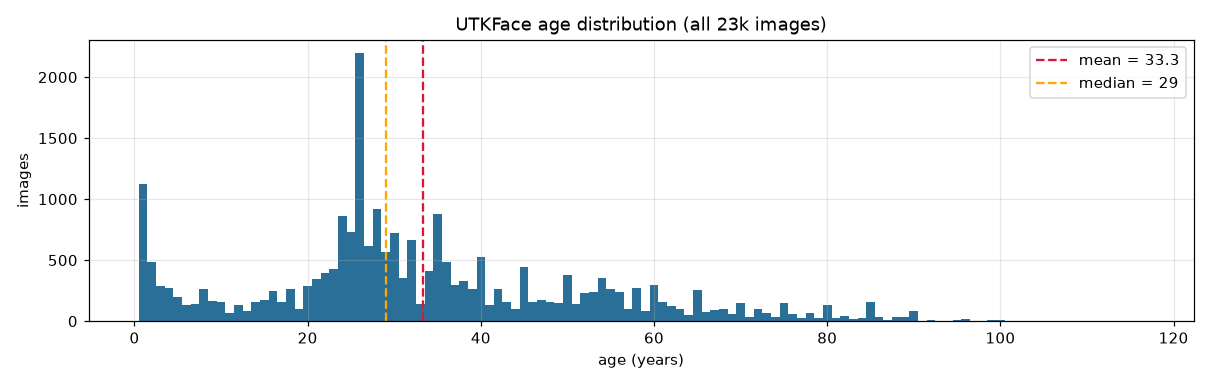
\includegraphics[width=\linewidth]{eda_age_hist.png}
\caption{Age distribution of UTKFace. Most images show people aged 20--39; round ages above 40 occur 2.4--5.9$\times$ more often than their neighbours (label heaping).}
\label{fig:agehist}
\end{figure}

\subsection{Input and baseline}
All models see the native $3\times200\times200$ image (no resizing, the same policy for every model), scaled to $[0,1]$ and normalised with the ImageNet mean and standard deviation. Predicting the mean training age (33.23) gives a test MAE of $\mathrm{MAE}_{\text{mean}} = 15.40$ (RMSE 20.01); the median (29) gives 15.07. Hence the second condition of~\eqref{eq:accept} is $\mathrm{MAE}_{\text{own}} \le 9.24$.

% =====================================================================
\section{Our CNN}
\label{sec:own}
\subsection{Design}
Fig.~\ref{fig:own} shows the final network (next to the two standard models in Fig.~\ref{fig:archs}) and Table~\ref{tab:layers} gives every layer. In Fig.~\ref{fig:archs} each cuboid is a tensor (the output of a layer; height and depth $\propto\sqrt{H}$, width $\propto\log C$) and the operation that turns one tensor into the next is written in the gap between them: the operation (bold), what follows it inside the same layer (BN = BatchNorm, ReLU), and its stride S and padding P. S\,=\,2 means the kernel moves two pixels at a time, so $H$ and $W$ are halved, e.g.\ ResNet18's first conv ($k=7$, S\,=\,2, P\,=\,3): $\lfloor(200+2\cdot3-7)/2\rfloor+1=100$; S\,=\,1 with P\,=\,$\lfloor k/2\rfloor$ keeps the size. The red square is the $k\times k$ kernel on the tensor it slides over, and arcs are shortcuts: \emph{identity} (no parameters) or \emph{projection} ($1\times1$ stride-2 convolution). The numbers under each cuboid are conv weights only for our CNN and ResNet18 and whole blocks for MobileNetV3. All shapes come from forward hooks on the real models. The design follows four ideas.

\emph{Terms used in Fig.~\ref{fig:archs}.} The \textbf{stem} is the first part of a network, before the repeated blocks: it turns the $3\times200\times200$ image into a smaller feature map so that the expensive blocks work on fewer positions (ours: $3\times3$ stride-2 conv + $3\times3$ stride-2 max pool, $200\to50$; ResNet18: $7\times7$ stride-2 conv + max pool, $200\to50$; MobileNetV3: one $3\times3$ stride-2 conv, $200\to100$). A \textbf{shortcut} (skip connection) is the second path of a residual block: the block input $x$ goes around the convolutions $F$ and is added to their output, $y=\mathrm{ReLU}(F(x)+S(x))$, drawn as an arc ending in $\oplus$. There are two kinds. An \textbf{identity shortcut} passes $x$ unchanged, $S(x)=x$, and has no parameters; it is possible only when $F(x)$ has the same shape as $x$. A \textbf{projection shortcut} is used in the first block of a stage, where $F$ halves $H$ and $W$ and doubles $C$, so $x$ no longer fits: $S(x)$ is a $1\times1$ stride-2 convolution plus BatchNorm that reshapes $x$ to the new size (e.g.\ stage 2 of our CNN: $32\times50\times50\to64\times25\times25$ with $32\cdot64 = 2{,}048$ weights). So ``projection'' is a kind of shortcut, not an alternative to it. In MobileNetV3 the unlabelled $\oplus$ arcs are identity shortcuts; its blocks that change shape have no shortcut at all.

\emph{Shrink early.} A $3\times3$ stride-2 convolution and a $3\times3$ stride-2 max pool reduce $200\times200$ to $50\times50$ before any wide layer, because the cost of a convolution grows with $H\times W$. With $H_{\text{out}} = \lfloor (H + 2p - k)/s \rfloor + 1$, the stem gives $\lfloor(200+2-3)/2\rfloor+1 = 100$ and the pool $\lfloor(100+2-3)/2\rfloor+1 = 50$.

\emph{Residual stages.} Four stages with 32, 64, 128 and 256 channels (half of ResNet18's 64--512, so each $3\times3$ conv has a quarter of the parameters, since params $\propto C_{\text{in}}C_{\text{out}}$) each contain two basic blocks: $y = \mathrm{ReLU}(F(x) + S(x))$ with $F$ = conv$3\times3$--BN--ReLU--conv$3\times3$--BN. The first block of stages 2--4 halves $H$ and $W$ with stride 2 and doubles the channels, so its shortcut $S$ is a $1\times1$ stride-2 convolution with BatchNorm (projection); all other shortcuts are identities without parameters. Stride-2 on the first conv keeps the total cost per stage roughly constant, since halving $H$ and $W$ divides MACs by 4 while doubling both $C_{\text{in}}$ and $C_{\text{out}}$ multiplies them by 4.

\emph{Non-linearity.} Every convolution is followed by BatchNorm and ReLU~\cite{nair2010relu}, except the second convolution of each block, whose ReLU comes after the addition (``BN only'' and ``ReLU'' next to $\oplus$ in Fig.~\ref{fig:own}). The network therefore has 17 ReLUs (one in the stem and two in each of the 8 blocks) plus the max pool. They are what makes it deep: convolutions, BatchNorm at inference, average pooling and the head are all linear, and without activations any stack of them collapses into a single linear map, $W_2(W_1x) = (W_2W_1)x$. With ReLUs the network is piecewise linear with a very large number of regions. We chose ReLU rather than GELU~\cite{hendrycks2016gelu} or (hard-)swish because it is the cheapest activation (a comparison, whose gradient is a 0/1 mask), it matches Kaiming initialisation (gain $\sqrt{2}$) and ResNet18's block, so the comparison with ResNet18 changes only width and depth, and replacing ReLU with GELU did not change ImageNet accuracy in ConvNeXt~\cite{liu2022convnext}. We did not test other activations, to save a training run.

\emph{Global average pooling head.} The $256\times7\times7$ map is averaged to 256 features~\cite{lin2014nin} and a Linear(256,\,1) predicts the age. The network therefore needs only 257 head parameters and works at any input size.

\emph{Output scaling.} The head predicts a standardised age: $\hat{y} = \mu + \sigma\, f(x)$ with fixed (non-learned) $\mu = 33.23$ and $\sigma = 19.9$ from the training set. Without it, our first learning-rate search stayed at the baseline: the head starts near zero and Adam moves each weight by about one learning rate per step, so after 310 steps the predictions spread only 5--7 years instead of 19.9.

\begin{figure*}[p]
\centering
\begin{subfigure}{\textwidth}\centering
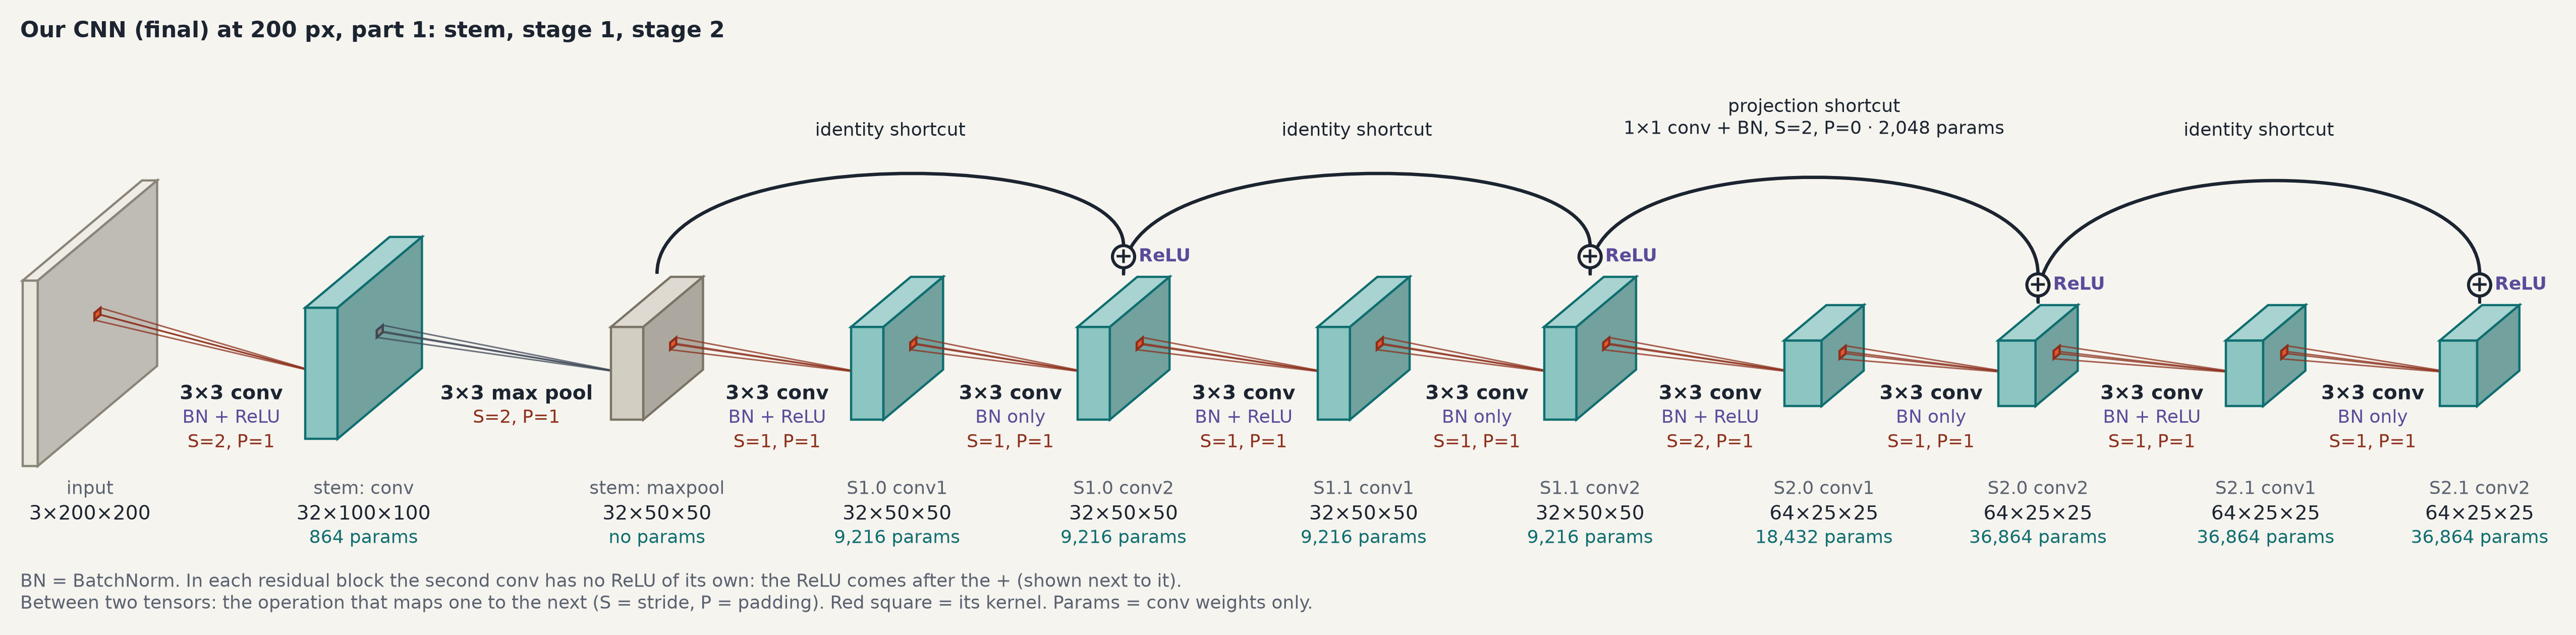
\includegraphics[width=0.95\textwidth]{own_cnn_final_part1.png}\\
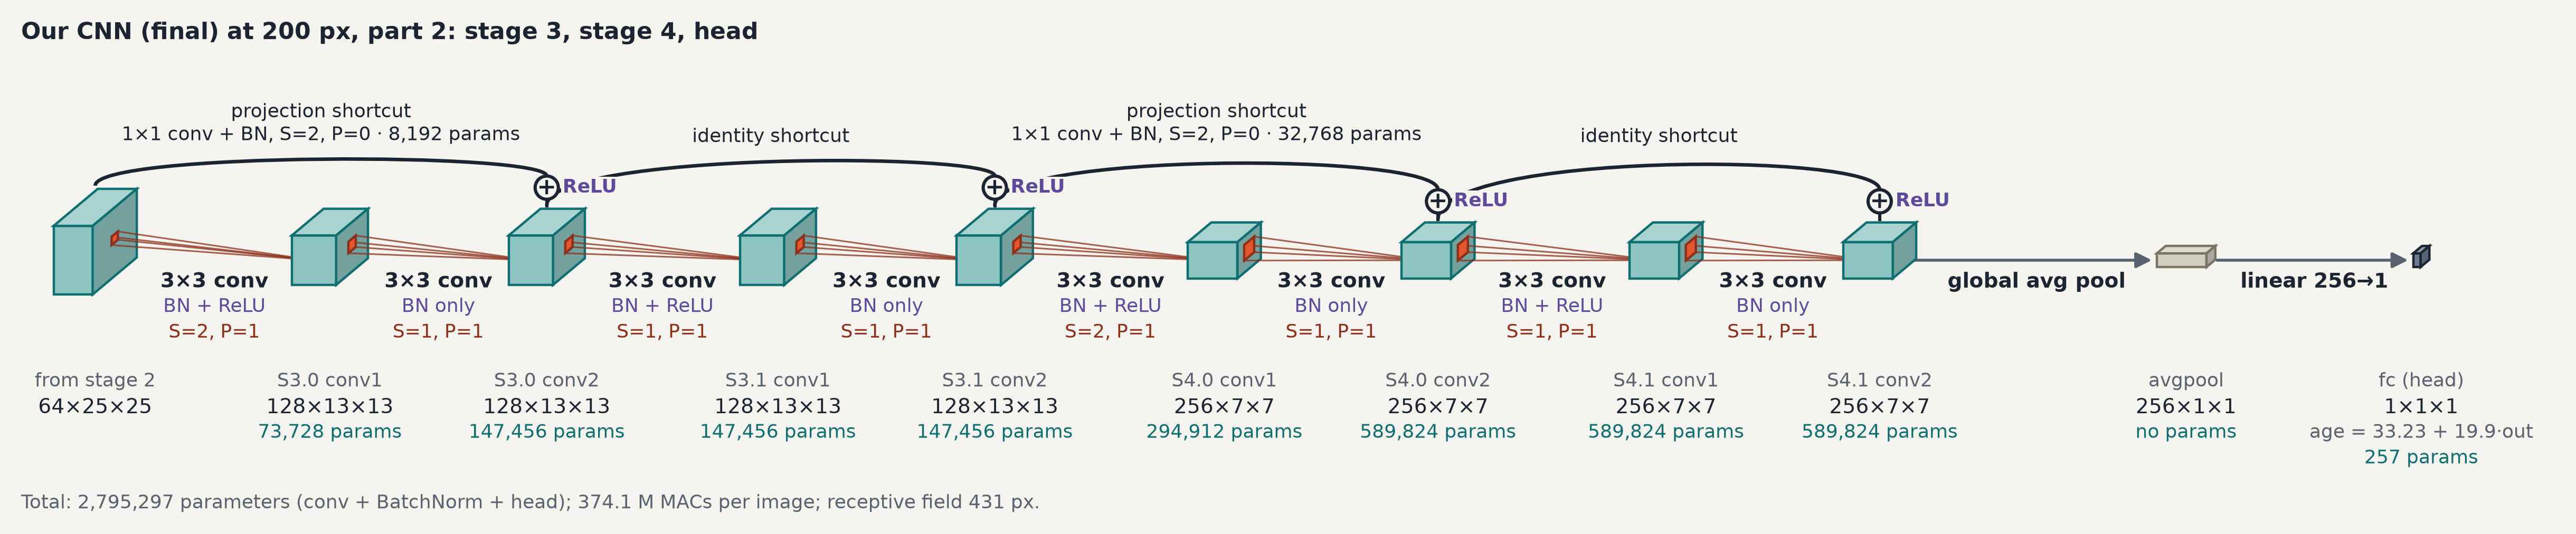
\includegraphics[width=0.95\textwidth]{own_cnn_final_part2.png}
\caption{Our CNN (final): 2 basic blocks per stage, 32--256 channels; 2.80\,M parameters, 374\,M MACs.}
\label{fig:own}
\end{subfigure}
\begin{subfigure}{\textwidth}\centering
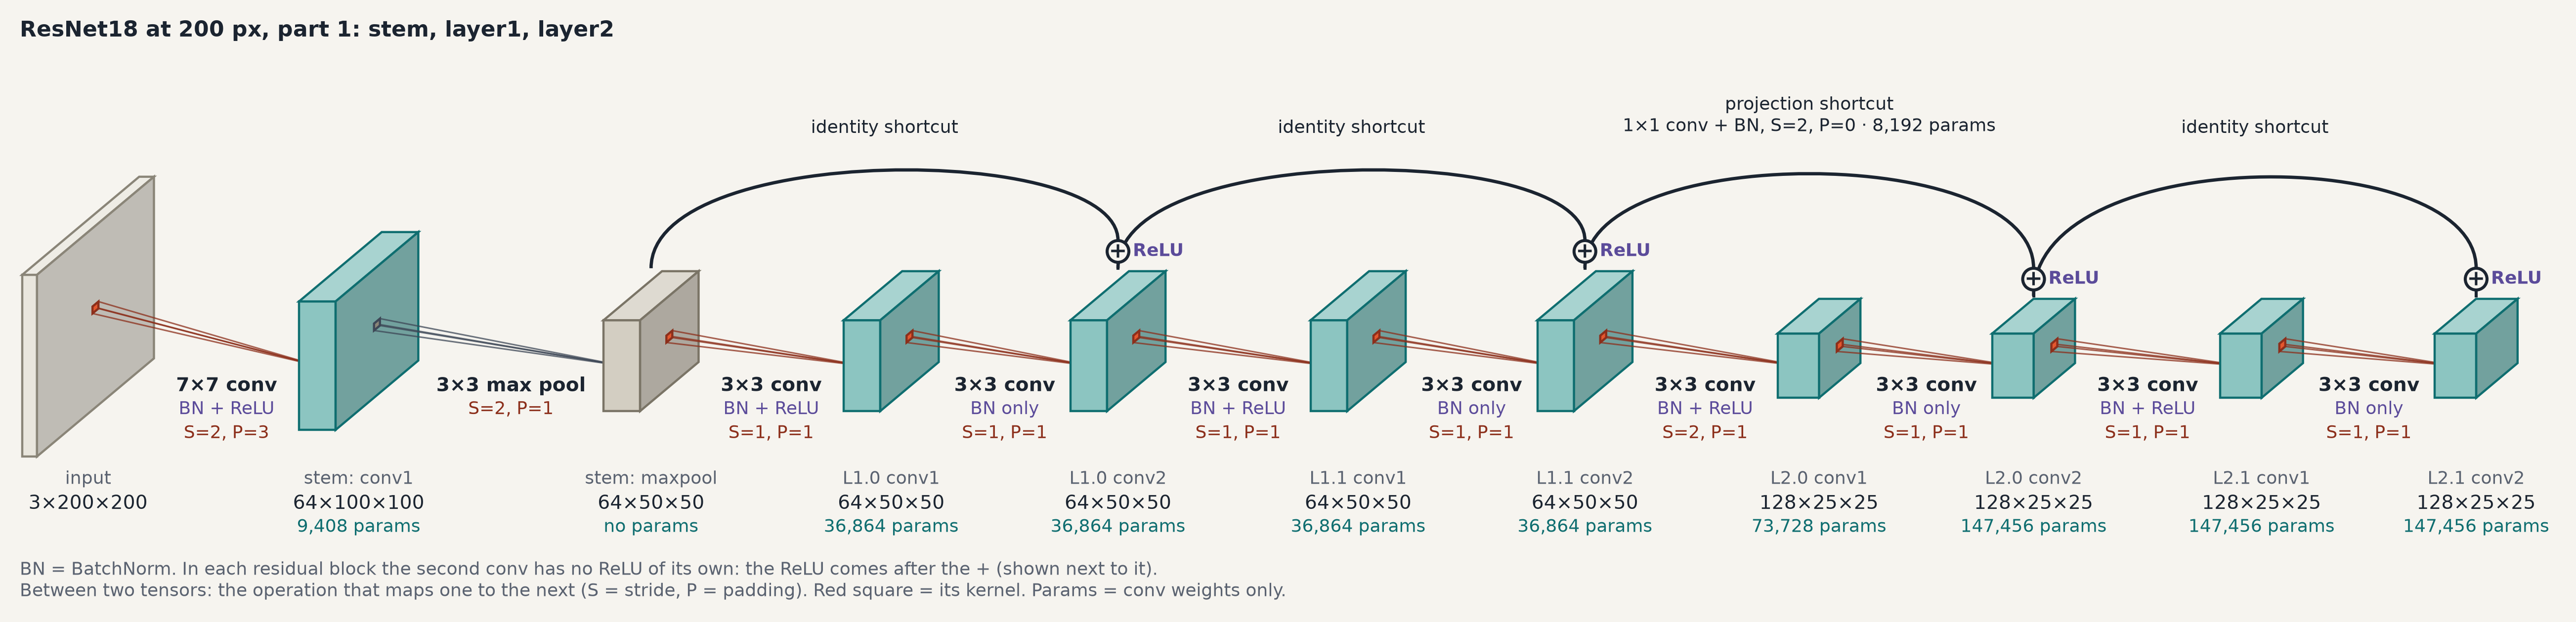
\includegraphics[width=0.95\textwidth]{resnet18_part1.png}\\
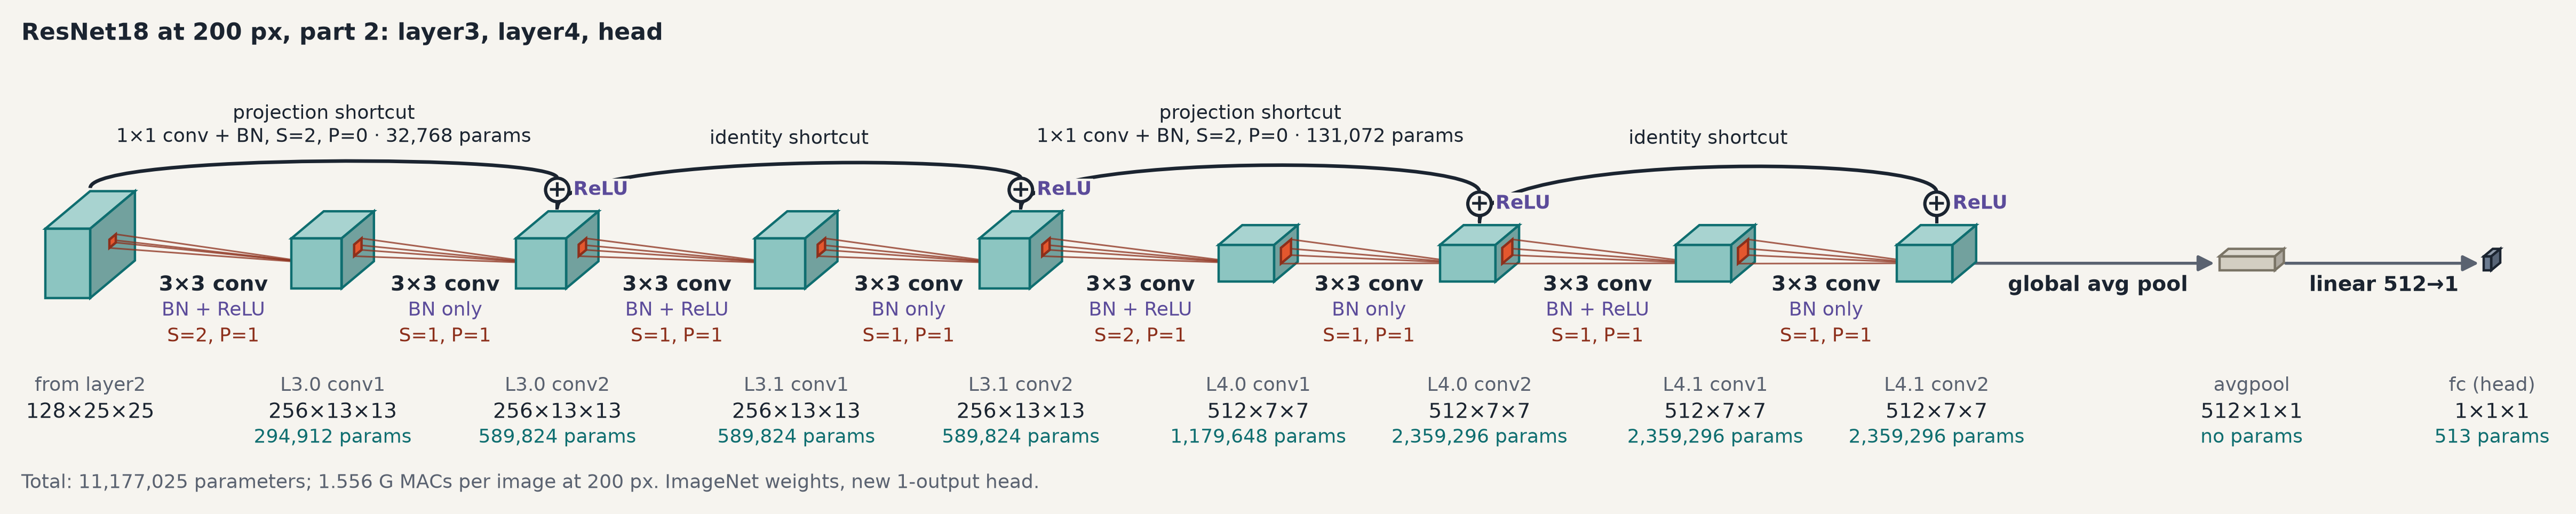
\includegraphics[width=0.95\textwidth]{resnet18_part2.png}
\caption{ResNet18: same 2-2-2-2 layout, $7\times7$ stem, twice the channels (64--512); 11.18\,M parameters (4$\times$), 1.556\,G MACs (4.2$\times$).}
\label{fig:resnet}
\end{subfigure}
\begin{subfigure}{\textwidth}\centering
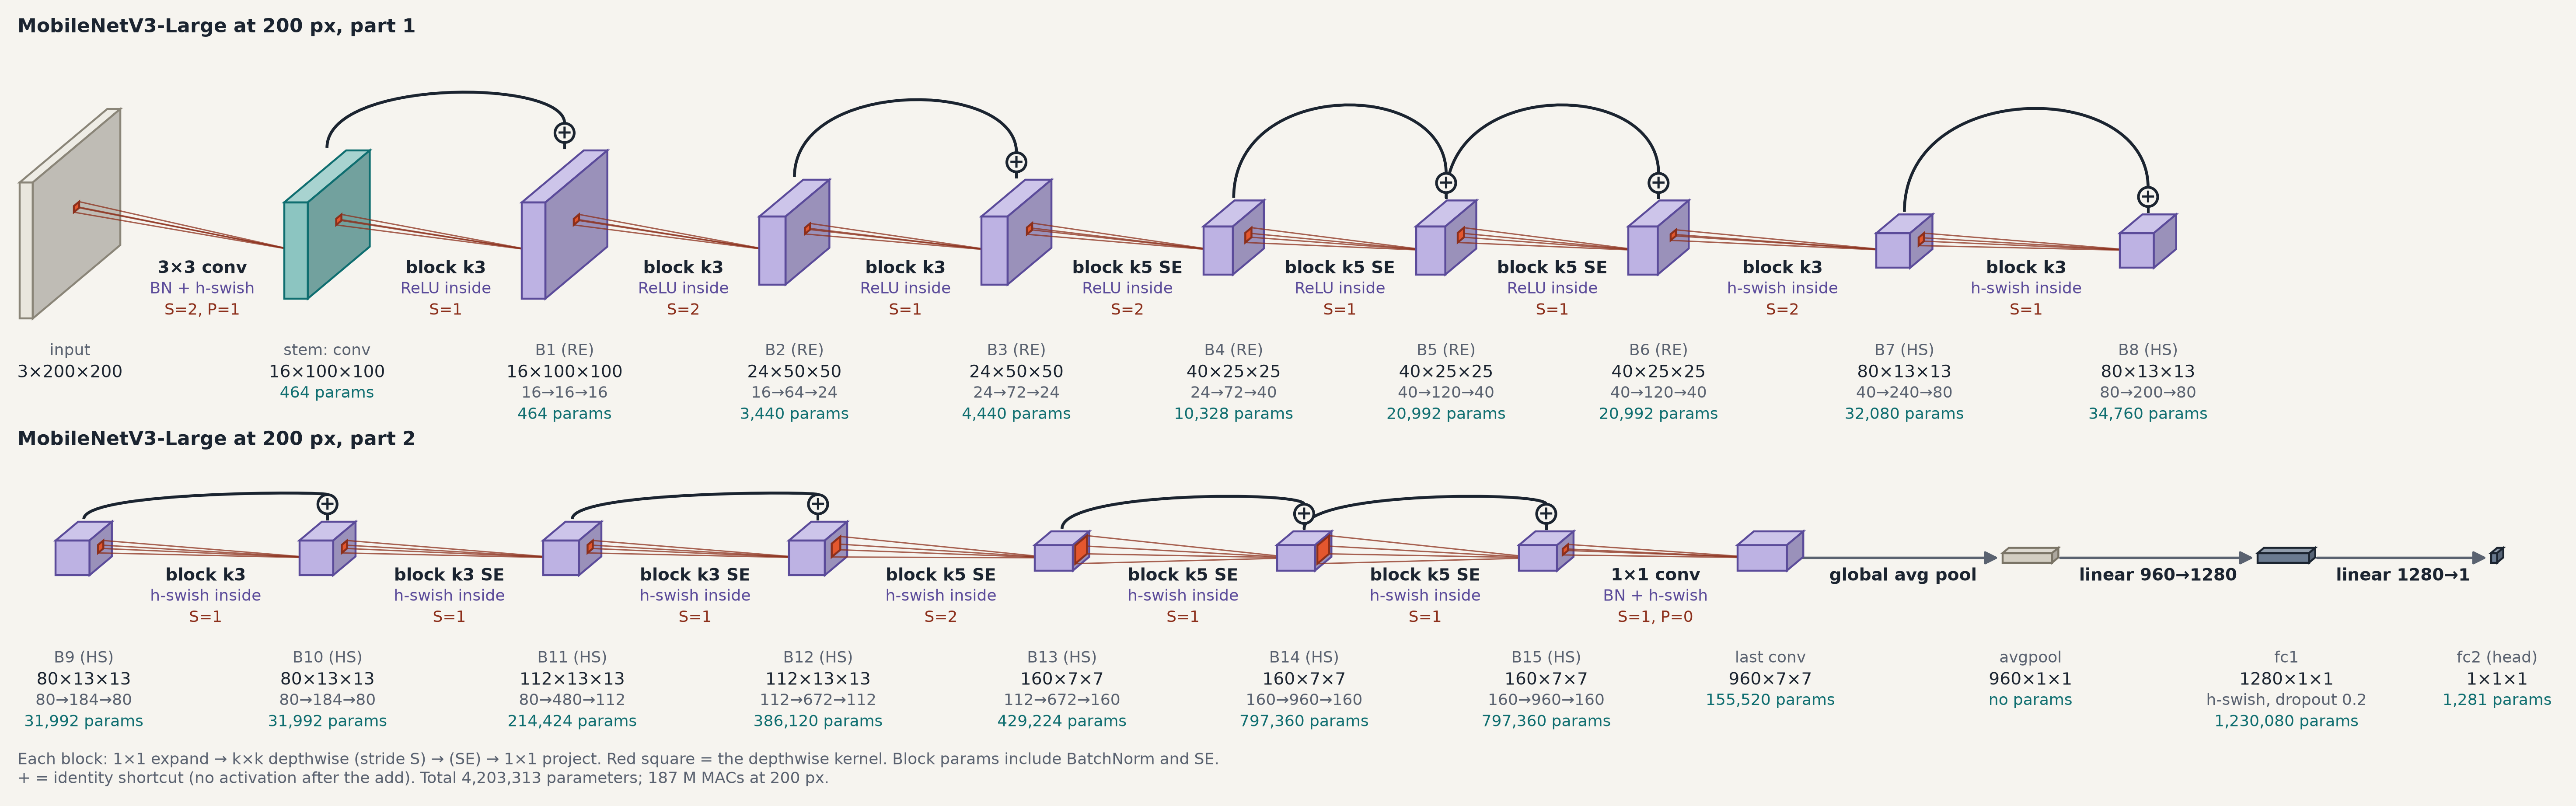
\includegraphics[width=0.95\textwidth]{mobilenet_v3_large.png}
\caption{MobileNetV3-Large, one cuboid per block; 4.20\,M parameters, 187\,M MACs.}
\label{fig:mnv3}
\end{subfigure}
\caption{The three trained architectures at the same 200\,px input and with the same drawing conventions (Section~\ref{sec:own}).}
\label{fig:archs}
\end{figure*}

\subsection{Per-layer analysis}
Table~\ref{tab:layers} uses
\begin{align*}
\text{params}_{\text{conv+BN}} &= C_{\text{in}} C_{\text{out}} k^2 + 2C_{\text{out}},\\
\text{MACs} &= H_{\text{out}} W_{\text{out}} C_{\text{out}} C_{\text{in}} k^2,\\
\text{RF}_{\text{new}} &= \text{RF}_{\text{old}} + (k-1)\,j, \quad j_{\text{new}} = j\cdot S,
\end{align*}
where $j$ is the jump (input pixels between neighbouring outputs). Convolutions have no bias because the following BatchNorm~\cite{ioffe2015bn} has its own shift; BN contributes $\gamma$ and $\beta$ per channel. For example, the stem has $3\cdot32\cdot9 + 64 = 928$ parameters and $100\cdot100\cdot32\cdot3\cdot9 = 8.64$\,M MACs, and its receptive field is $1 + 2\cdot1 = 3$ with jump 2. The total is 2{,}795{,}297 parameters and 374.1\,M MACs (748.2\,MFLOPs) per image; both were checked against PyTorch hooks. The receptive field reaches 431\,px after stage 4, i.e.\ every output position can see the whole 200\,px face.

\begin{table}[t]
\caption{Every layer of the final CNN (input $3\times200\times200$). $k$ = kernel size, S = stride, P = padding; params include BatchNorm; RF = receptive field in input pixels.}
\label{tab:layers}
\centering\scriptsize
\setlength{\tabcolsep}{3pt}
\begin{tabular}{@{}llrrrr@{}}
\toprule
Layer & $k$, S, P & Output & Params & MACs (M) & RF \\
\midrule
stem conv & 3, 2, 1 & $32\times100\times100$ & 928 & 8.64 & 3 \\
max pool & 3, 2, 1 & $32\times50\times50$ & 0 & -- & 7 \\
S1.0 conv1, conv2 & 3, 1, 1 & $32\times50\times50$ & 2$\times$9{,}280 & 2$\times$23.04 & 15, 23 \\
S1.1 conv1, conv2 & 3, 1, 1 & $32\times50\times50$ & 2$\times$9{,}280 & 2$\times$23.04 & 31, 39 \\
S2.0 conv1 & 3, 2, 1 & $64\times25\times25$ & 18{,}560 & 11.52 & 47 \\
S2.0 conv2 & 3, 1, 1 & $64\times25\times25$ & 36{,}992 & 23.04 & 63 \\
S2.0 shortcut & 1, 2, 0 & $64\times25\times25$ & 2{,}176 & 1.28 & -- \\
S2.1 conv1, conv2 & 3, 1, 1 & $64\times25\times25$ & 2$\times$36{,}992 & 2$\times$23.04 & 79, 95 \\
S3.0 conv1 & 3, 2, 1 & $128\times13\times13$ & 73{,}984 & 12.46 & 111 \\
S3.0 conv2 & 3, 1, 1 & $128\times13\times13$ & 147{,}712 & 24.92 & 143 \\
S3.0 shortcut & 1, 2, 0 & $128\times13\times13$ & 8{,}448 & 1.38 & -- \\
S3.1 conv1, conv2 & 3, 1, 1 & $128\times13\times13$ & 2$\times$147{,}712 & 2$\times$24.92 & 175, 207 \\
S4.0 conv1 & 3, 2, 1 & $256\times7\times7$ & 295{,}424 & 14.45 & 239 \\
S4.0 conv2 & 3, 1, 1 & $256\times7\times7$ & 590{,}336 & 28.90 & 303 \\
S4.0 shortcut & 1, 2, 0 & $256\times7\times7$ & 33{,}280 & 1.61 & -- \\
S4.1 conv1, conv2 & 3, 1, 1 & $256\times7\times7$ & 2$\times$590{,}336 & 2$\times$28.90 & 367, 431 \\
global avg pool & 7, 1, 0 & $256$ & 0 & -- & -- \\
fc (head) & -- & 1 & 257 & $<$0.01 & -- \\
\midrule
\textbf{Total} & & & \textbf{2{,}795{,}297} & \textbf{374.1} & \textbf{431} \\
\bottomrule
\end{tabular}
\end{table}

\subsection{Training setup and justification}
\label{sec:owntrain}
\emph{Loss and metric:} L1 loss, so training optimises the reported MAE and is less sensitive than MSE to noisy labels of old people. \emph{Initialisation:} Kaiming normal~\cite{he2015delving} for convolutions; the last BN $\gamma$ of every residual branch starts at 0, so each block starts as its shortcut and the untrained network behaves like a shallow one~\cite{goyal2017accurate}. \emph{Optimiser:} AdamW~\cite{loshchilov2019adamw}, weight decay 0.01, batch 128, one linear warm-up epoch followed by cosine decay to zero~\cite{loshchilov2017sgdr}, bf16 mixed precision~\cite{micikevicius2018mixed}. \emph{Learning rate:} chosen on a 4{,}000-image subset (10 epochs each); validation MAE was 11.87, 10.42 and 10.01 for $10^{-3}$, $3\cdot10^{-3}$ and $10^{-2}$, so we used $10^{-2}$. \emph{Augmentation} (identical for all models, training only): horizontal flip ($p=0.5$), rotation $\pm10^{\circ}$ and shift $\pm8$\,px in one bilinear resampling with black fill, greyscale ($p=0.1$). \emph{Regularisation:} weight decay, augmentation and BatchNorm; no dropout. \emph{Stopping:} a fixed epoch budget, keeping the weights of the best validation epoch.

\subsection{From the first version to the final model}
The first version had one block per stage (1.23\,M parameters, 174.3\,M MACs, RF 191) and reached a validation MAE of 5.79 and a test MAE of 5.77 after 40 epochs, \emph{not} acceptable (limit 5.48). Its training loss (5.23) was close to the validation MAE and still falling (Fig.~\ref{fig:d2}), i.e.\ it was underfitting. We therefore added a second block per stage (ResNet18's 2-2-2-2 layout) and trained 60 instead of 40 epochs. To save a run, both changes were made at once, so their individual effects cannot be separated. The final model reached a validation MAE of 5.145 and a test MAE of 5.140. The last 20 epochs improved validation by only 0.03 years while the training loss fell from 4.39 to 3.81, so we did not train longer.

\begin{figure}[t]
\centering
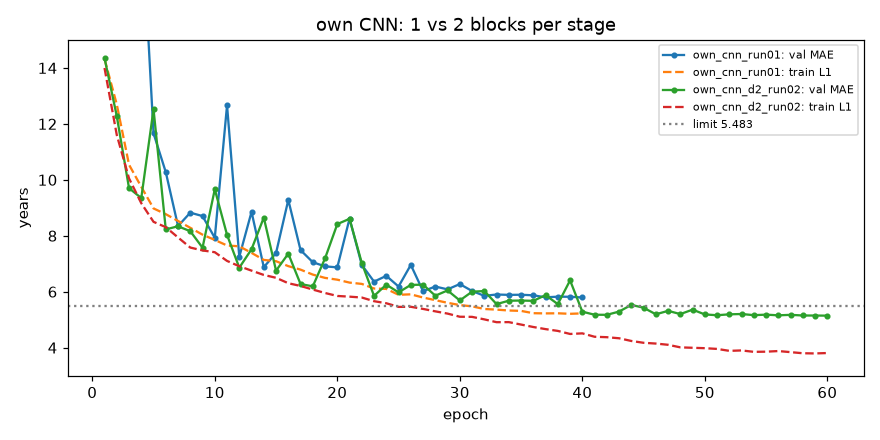
\includegraphics[width=\linewidth]{own_cnn_d2_vs_run01.png}
\caption{Training L1 loss and validation MAE of our CNN with 1 block per stage (40 epochs) and 2 blocks per stage (60 epochs). The dotted line is the acceptability limit 5.483. Validation is noisy while the learning rate is high and settles under cosine decay.}
\label{fig:d2}
\end{figure}

\subsection{Ablation: basic vs.\ bottleneck blocks}
\label{sec:ablation}
As the required ablation we changed \emph{one} design choice of the first version and kept everything else (40 epochs, same data, seed and schedule): the basic block was replaced by a bottleneck block~\cite{he2016resnet} ($1\times1$ to $C/4$, $3\times3$, $1\times1$ back to $C$; Fig.~\ref{fig:bottle}). Table~\ref{tab:ablation} and Fig.~\ref{fig:ablation} show the result. The bottleneck network has 10$\times$ fewer parameters and 6.6$\times$ fewer MACs, but its error is 1.67 years higher (test 7.43) and it saved only 7\,\% of the energy per epoch. Both networks ran at about 1.2\,s per epoch, the time of our data pipeline (augmentation on the GPU, batch loading): below that point, a smaller model no longer reduces energy. Its receptive field (71\,px) is also much smaller than the face, because only one of its three convolutions per block is $3\times3$.

\begin{figure}[t]
\centering
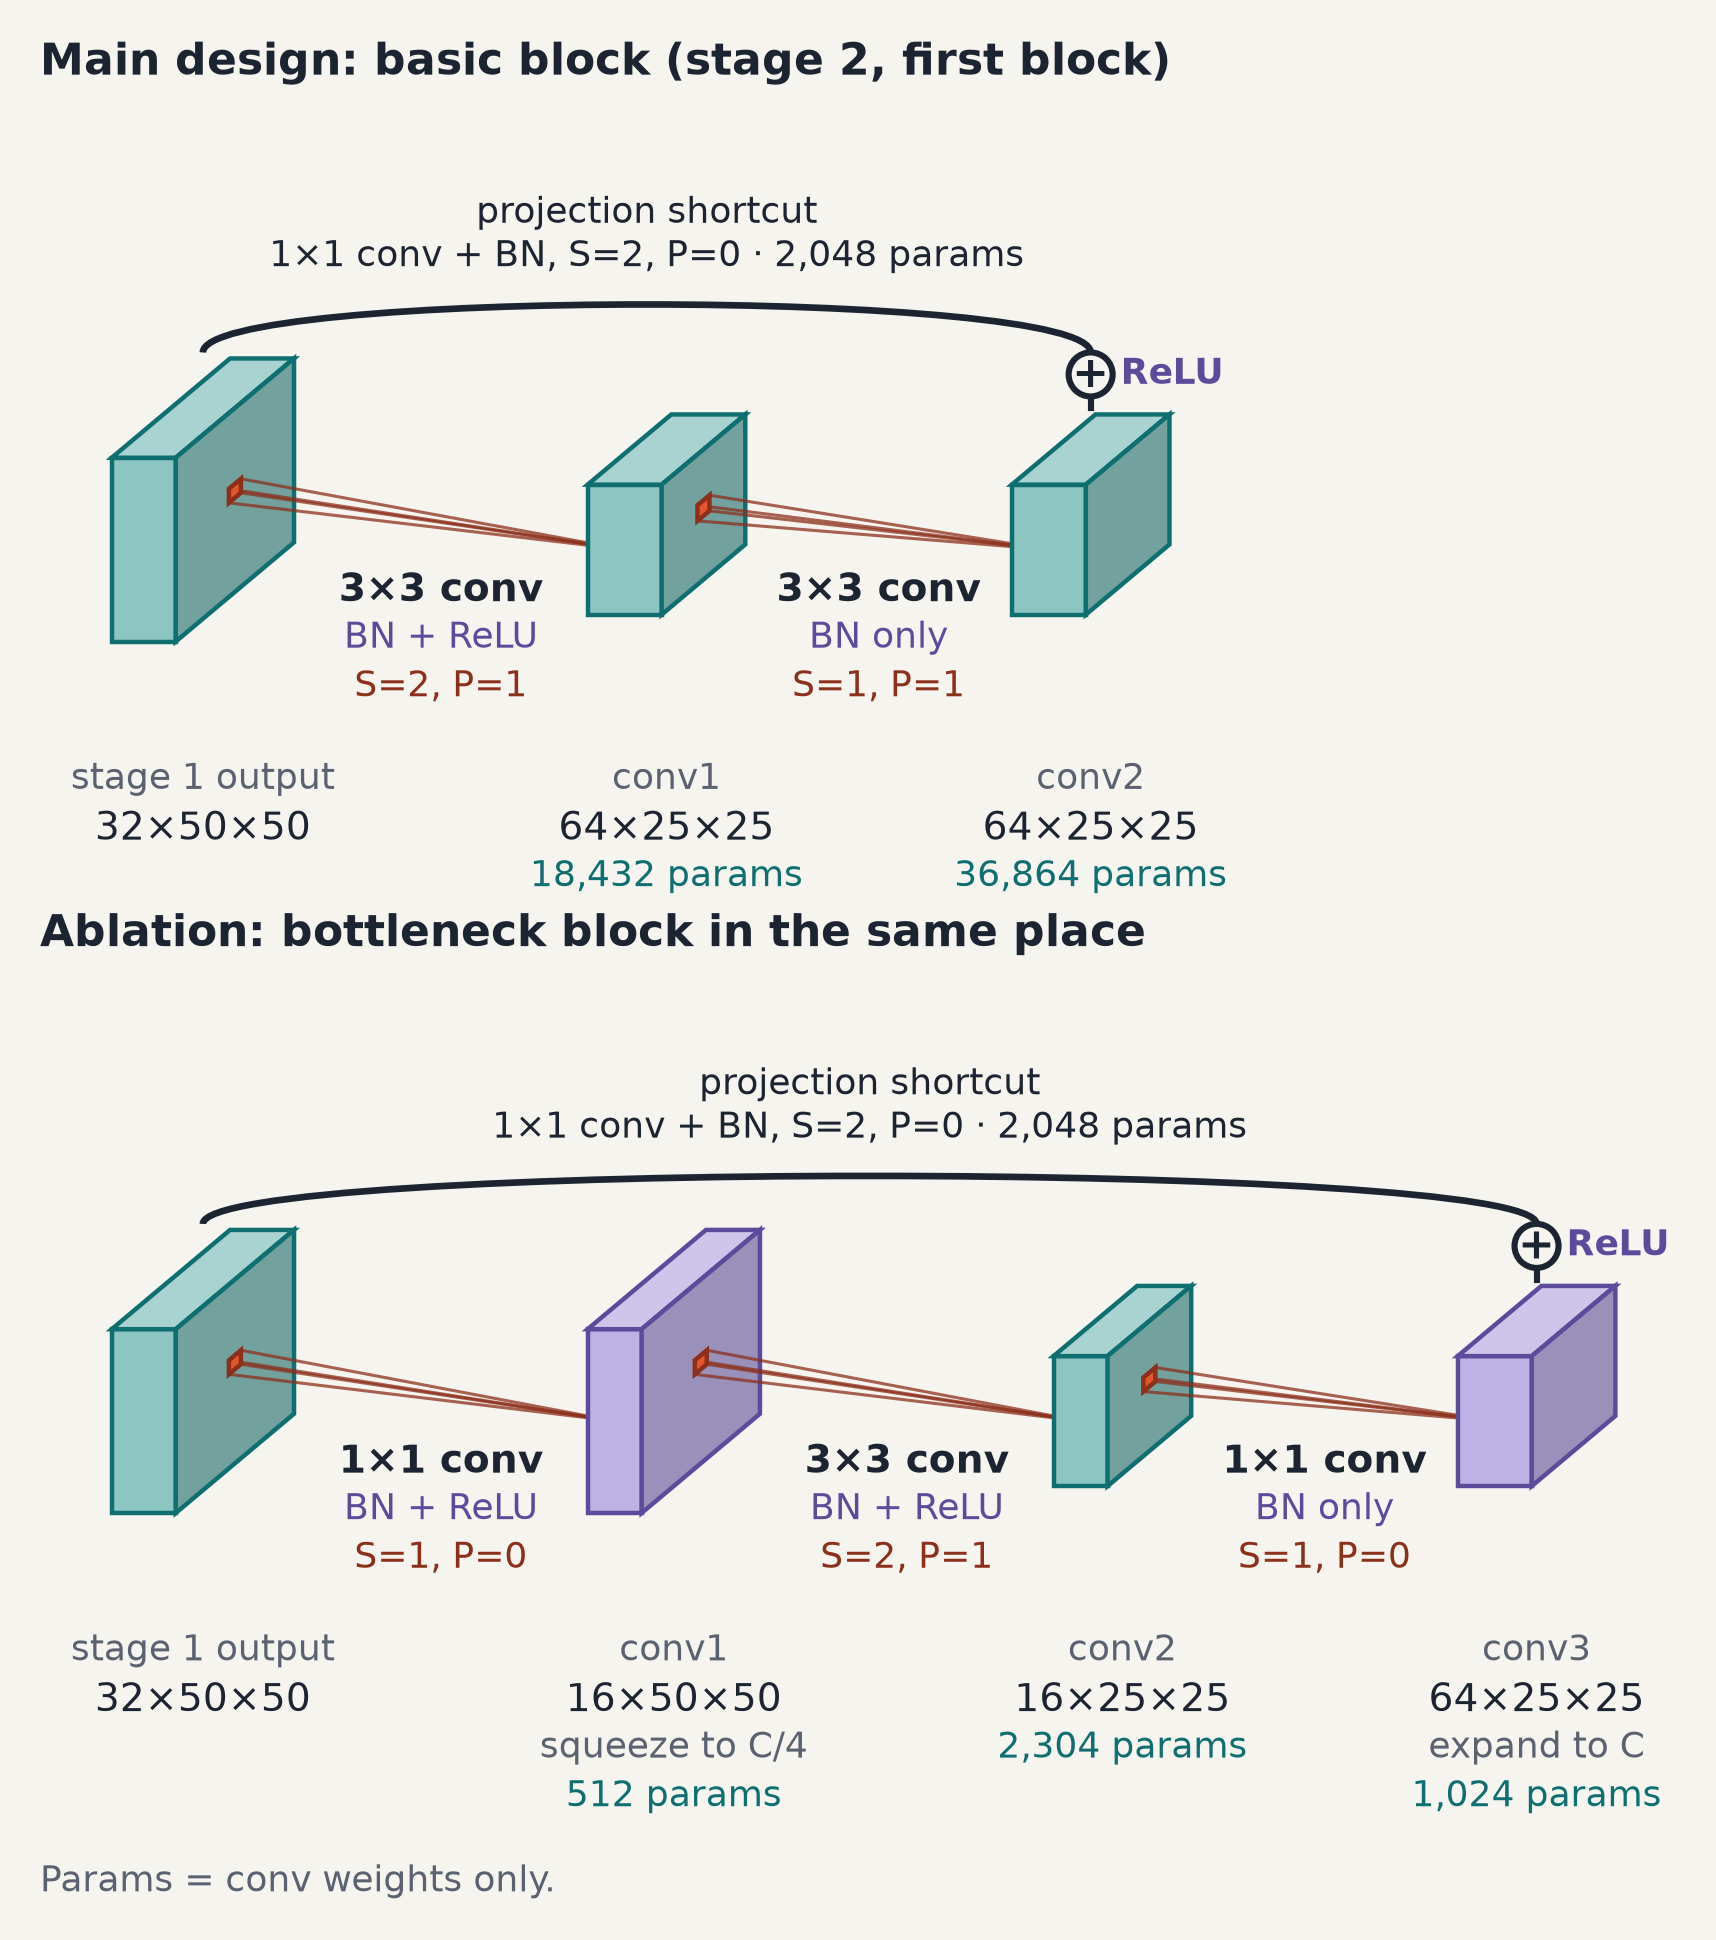
\includegraphics[width=0.78\linewidth]{own_cnn_bottleneck.png}
\caption{Ablation: the first block of stage 2 as a basic block (main design, top) and as a bottleneck block (bottom). Purple = $1\times1$ convolutions.}
\label{fig:bottle}
\end{figure}

\begin{table}[t]
\caption{Ablation on the 1-block-per-stage network (40 epochs each).}
\label{tab:ablation}
\centering\footnotesize
\setlength{\tabcolsep}{4pt}
\begin{tabular}{@{}lrr@{}}
\toprule
 & Basic (main) & Bottleneck \\
\midrule
Parameters & 1{,}226{,}657 & 128{,}257 \\
MACs per image & 174.3\,M & 26.5\,M \\
Receptive field & 191\,px & 71\,px \\
Validation / test MAE & 5.794 / 5.765 & 7.366 / 7.434 \\
Training energy & 5.12\,Wh & 4.77\,Wh \\
Training emissions & 2.38\,g & 2.22\,g \\
Time per epoch & 1.17\,s & 1.24\,s \\
\bottomrule
\end{tabular}
\end{table}

\begin{figure}[t]
\centering
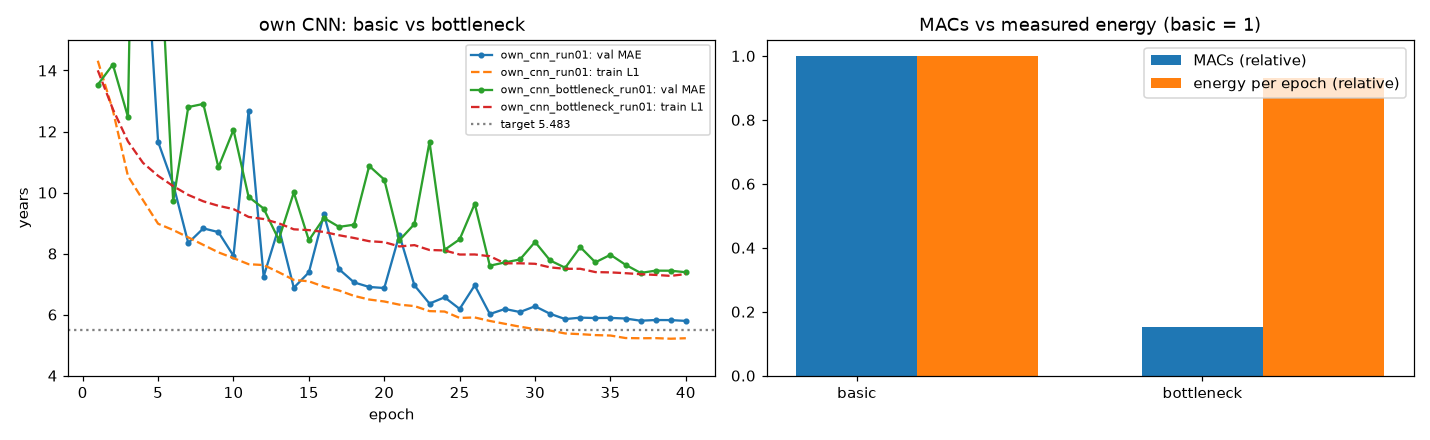
\includegraphics[width=\linewidth]{own_cnn_ablation_bottleneck.png}
\caption{Ablation curves (left) and relative MACs vs.\ measured energy per epoch (right): 85\,\% fewer MACs give only 7\,\% less energy.}
\label{fig:ablation}
\end{figure}

% =====================================================================
\section{Standard Models}
\label{sec:standard}
We fine-tune two torchvision models from their ImageNet (V1) weights~\cite{paszke2019pytorch}: ResNet18~\cite{he2016resnet} as the large model (11.18\,M parameters, 1.556\,G MACs at 200\,px; Fig.~\ref{fig:resnet}) and MobileNetV3-Large~\cite{howard2019mobilenetv3} as the efficiency-oriented model (4.20\,M parameters, 0.187\,G MACs; Fig.~\ref{fig:mnv3}, where block labels give the kernel size, SE = squeeze-and-excitation, /2 = stride 2, RE/HS = ReLU/hard-swish and input$\to$expanded$\to$output channels; most of its parameters sit in the last $1\times1$ conv and the 960$\to$1280 head layer). In both, the 1000-class layer is replaced by a single-output Linear layer with zero weights and bias 33.23 (the mean age), so training starts at the baseline. Both take the same 200\,px input, which works because a global average pool sits before the head.
Two strategies were trained for each model, 15 epochs, batch 128, bf16, L1, AdamW with weight decay 0.01, the augmentation of Section~\ref{sec:owntrain}, and the best validation epoch kept:
\begin{itemize}
\item \textbf{A (partial):} one epoch training only the head (lr $10^{-3}$), then the last layers (ResNet18: \texttt{layer3}, \texttt{layer4}; MobileNetV3: blocks 7--16), head lr $10^{-3}$ and backbone lr $10^{-4}$ with cosine decay; the early layers stay frozen with their BatchNorm in evaluation mode.
\item \textbf{Full:} all layers from the first epoch with the same learning rates.
\end{itemize}
A first attempt with early stopping (patience 3) stopped ResNet18 while it was still improving at a low learning rate, so all final runs use the fixed 15-epoch budget. Full fine-tuning was better on validation for both models (ResNet18 4.761 vs.\ 4.993; MobileNetV3 5.092 vs.\ 5.242) at about 1.9$\times$ the energy.

% =====================================================================
\section{Measuring the Footprint}
\label{sec:footprint}
\emph{Hardware and location.} All reported runs ran on one lab machine in T\"urkiye: AMD Ryzen~9 9950X3D, NVIDIA RTX~5090 (32\,GB, \texttt{cuda:0}), Ubuntu 24.04, PyTorch 2.15 (CUDA 13.2). Small development steps on a laptop and a MacBook involved no training and are not counted.

\emph{Tool.} Every training, evaluation, test, search, cache-building and failed run is wrapped in CodeCarbon 3.3.2~\cite{codecarbon} (\texttt{OfflineEmissionsTracker}, country code TUR, grid intensity 465\,g~\cotwoeq/kWh). CodeCarbon samples GPU power through NVML, CPU power, and RAM power, integrates them over time, and multiplies the energy by the grid intensity. The lab machine is shared with other users, so we (i) measure only GPU~0, (ii) use CodeCarbon's \emph{process} mode for CPU and RAM, so other users' processes are not charged to us, and (iii) log any foreign process found on our GPU. All logs are in \texttt{logs/emissions/emissions.csv} (CodeCarbon) and \texttt{logs/runs.csv} (one row per run).

\emph{Inference metrics.} Latency is the mean time per image at batch size 1. Energy per 1{,}000 predictions is measured by repeating validation images at batch 512 for about 10\,s, because CodeCarbon samples power every few seconds and a single test pass lasts less than 1.5\,s.

\emph{Caveat.} On the last day another user's language model was running on GPU~0 at up to 254\,W. NVML reports the power of the whole board, so the energies of the final CNN's training run and inference benchmark are upper bounds. Epochs 12--40 of that run took 2.0\,s instead of 1.6\,s, which suggests the two jobs competed for the GPU.

% =====================================================================
\section{Results}
\label{sec:results}
\subsection{Main comparison}
Table~\ref{tab:results} is the main result. The best standard model is ResNet18 with full fine-tuning (test MAE 4.768), so the binding condition is $\mathrm{MAE}_{\text{own}} \le 1.15\times4.768 = 5.483$ (the second condition gives 9.24). Our final CNN reaches \textbf{5.140} and is \textbf{acceptable}, 0.34 years under the limit. The first version (5.765) and the bottleneck ablation (7.434) are not. Validation predicted test well for every model (differences $\le0.11$ years), confirming that the test set was not overfitted by our choices.

\begin{table*}[t]
\caption{Main results on the test set (3{,}461 images, each final model evaluated once). MFLOPs = $2\times$ MACs per image. Train = final training run; Project = all tracked runs of that architecture family, including searches, failed runs, tests and benchmarks.}
\label{tab:results}
\centering\footnotesize
\setlength{\tabcolsep}{4pt}
\begin{tabular}{@{}lrrrrrrrrrrr@{}}
\toprule
Model & Params & MFLOPs & Test & RMSE & $R^2$ & Train & Train & Project & ms/ & Wh/1000 & Size \\
 & & /img & MAE & & & kWh & kg \cotwoeq & kg \cotwoeq & img & pred. & MB \\
\midrule
Mean baseline & 0 & 0 & 15.400 & 20.007 & 0.000 & -- & -- & -- & -- & -- & -- \\
Median baseline & 0 & 0 & 15.072 & 20.471 & $-0.047$ & -- & -- & -- & -- & -- & -- \\
\midrule
ResNet18, A (partial) & 11{,}177{,}025 & 3111.7 & 4.888 & 6.996 & 0.878 & 0.00302 & 0.00140 & \multirow{2}{*}{0.00914$^{\dagger}$} & 0.80 & 0.0066 & 44.8 \\
\textbf{ResNet18, full} (best standard) & 11{,}177{,}025 & 3111.7 & \textbf{4.768} & 6.780 & 0.885 & 0.00571 & 0.00265 & & 0.80 & 0.0067 & 44.8 \\
MobileNetV3-L, A (partial) & 4{,}203{,}313 & 374.5 & 5.331 & 7.441 & 0.862 & 0.00405 & 0.00188 & \multirow{2}{*}{0.00881} & 2.18 & 0.0075 & 17.0 \\
MobileNetV3-L, full & 4{,}203{,}313 & 374.5 & 5.141 & 7.238 & 0.869 & 0.00753 & 0.00350 & & 2.12 & 0.0075 & 17.0 \\
\midrule
Own CNN, 1 block/stage & 1{,}226{,}657 & 348.6 & 5.765 & 8.118 & 0.835 & 0.00512 & 0.00238 & \multirow{3}{*}{0.01368} & 0.55 & 0.0019 & 4.9 \\
Own CNN, bottleneck (ablation) & 128{,}257 & 53.0 & 7.434 & 10.100 & 0.745 & 0.00477 & 0.00222 & & 0.63 & 0.0017 & 0.6 \\
\textbf{Own CNN, 2 blocks/stage (final)} & 2{,}795{,}297 & 748.2 & \textbf{5.140} & 7.424 & 0.862 & 0.01240 & 0.00576 & & 0.80 & 0.0027 & 11.2 \\
\bottomrule
\multicolumn{12}{@{}l}{\footnotesize $^{\dagger}$Includes the 2.62\,g balanced-loss experiment of Section~\ref{sec:bias}. Shared runs (cache, tests, baseline, bias evaluation: 1.83\,g) are not attributed to a family.}
\end{tabular}
\end{table*}

\begin{figure}[t]
\centering
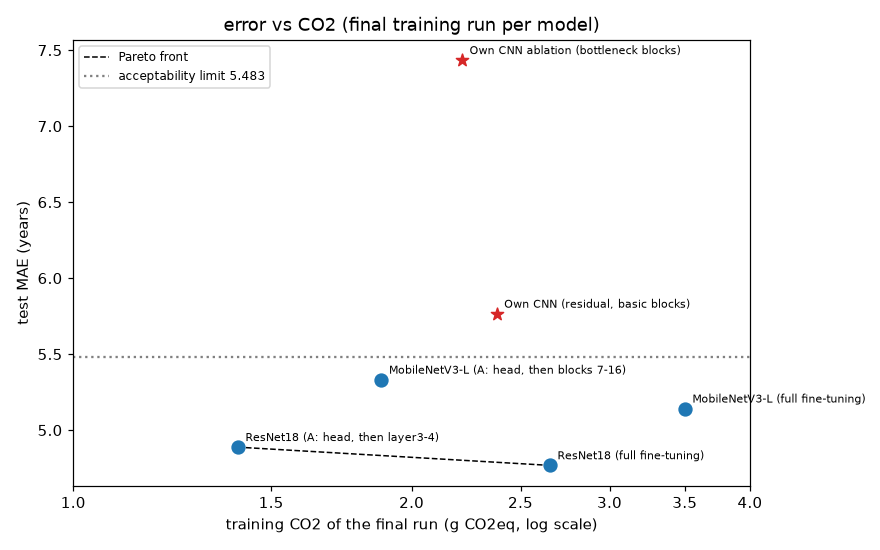
\includegraphics[width=\linewidth]{error_vs_co2_with_own_cnn.png}
\caption{Test MAE vs.\ \cotwo{} of the final training run (log scale), one point per configuration. The dashed line is the Pareto front (no other model is both more accurate and cheaper); the dotted line is the acceptability limit 5.483.}
\label{fig:pareto}
\end{figure}

\subsection{Error vs.\ \cotwo{}}
Fig.~\ref{fig:pareto} plots test MAE against the training emissions. On this axis the Pareto front consists only of the two ResNet18 runs: fine-tuning a pre-trained network for 15 epochs is both more accurate and cheaper than our 60-epoch training from scratch. Our final CNN is the most expensive training run (5.76\,g, 2.2$\times$ ResNet18 full), and over the whole project our CNN family cost 13.68\,g against 9.14\,g for ResNet18 and 8.81\,g for MobileNetV3. Two facts change this picture:
\begin{enumerate}
\item \emph{Inference.} Our CNN needs 0.0027\,Wh per 1{,}000 predictions vs.\ 0.0067 for ResNet18 and 0.0075 for MobileNetV3. Its extra training energy (12.40$-$5.71 = 6.69\,Wh) is repaid after $6.69/0.0040 \approx 1.7$ million predictions; a deployed model passes this point quickly. In inference energy our CNN dominates MobileNetV3 (same MAE, 2.8$\times$ less energy).
\item \emph{Pre-training is not free.} The ResNet18 weights were trained on ImageNet's 1.28\,M images for 90 epochs at 224\,px. Relative to our 15-epoch fine-tuning this is $79\times$ the images, $1.25\times$ the pixels and $6\times$ the epochs, about $600\times$ the work. On our GPU that would be roughly $600\times5.7\,\text{Wh}\approx3.4$\,kWh $\approx1.6$\,kg~\cotwoeq, about 600 times the fine-tuning run. This cost is shared by everyone who downloads the weights, so it is fair to amortise it, but it is not zero; MobileNetV3's 600-epoch recipe is even more costly.
\end{enumerate}

\subsection{Where the energy went}
Of the 72.0\,Wh measured in total, training runs used 54.3\,Wh (75\,\%), evaluations and inference benchmarks 11.3\,Wh (16\,\%), code tests 4.1\,Wh, learning-rate searches 2.2\,Wh and building the image cache 0.15\,Wh. The GPU accounted for 96\,\% of the energy. The inference benchmarks were costly compared with the test passes themselves (about 1.5\,Wh each vs.\ 0.04\,Wh for a test pass), because they must run long enough for CodeCarbon to sample.

\subsection{MACs are not energy}
Fig.~\ref{fig:findings}(b) in the appendix shows that MobileNetV3-L has 8$\times$ fewer FLOPs than ResNet18 but used 1.3$\times$ more energy per full fine-tuning epoch (0.502 vs.\ 0.381\,Wh) and is 2.7$\times$ slower at batch size 1. Depthwise convolutions do little arithmetic per byte moved, so they are limited by memory bandwidth and kernel launches rather than by the GPU's matrix units. The same effect appeared twice more: freezing the early layers (strategy A) saved 1.9$\times$ energy per epoch although it removes only a third of the backward MACs, because the early, high-resolution layers are memory-heavy; and the bottleneck ablation cut MACs by 85\,\% but energy by only 7\,\%.

% =====================================================================
\section{Bias Analysis}
\label{sec:bias}
\textbf{By age.} Fig.~\ref{fig:agemae} shows the test MAE per age band. All models are accurate for babies (about 1 year at 0--2) and their error grows with age, up to 9--11 years at 80+. Our CNN is within 2--8\,\% of ResNet18 in most bands, better at 0--2 (0.97 vs.\ 1.19), and weakest at 3--12 (+28\,\%), 50--59 and 80+ (+16\,\%). Fig.~\ref{fig:valbias} (validation set) shows that the error is not a global ``too old'' bias but a \emph{regression to the mean}: people younger than about 30 are predicted too old and older people too young (ResNet18: $+2.5$ years at 13--19, $-7.6$ at 80+), with the bias growing with the distance from the dense 20--39 region.

\begin{figure}[t]
\centering
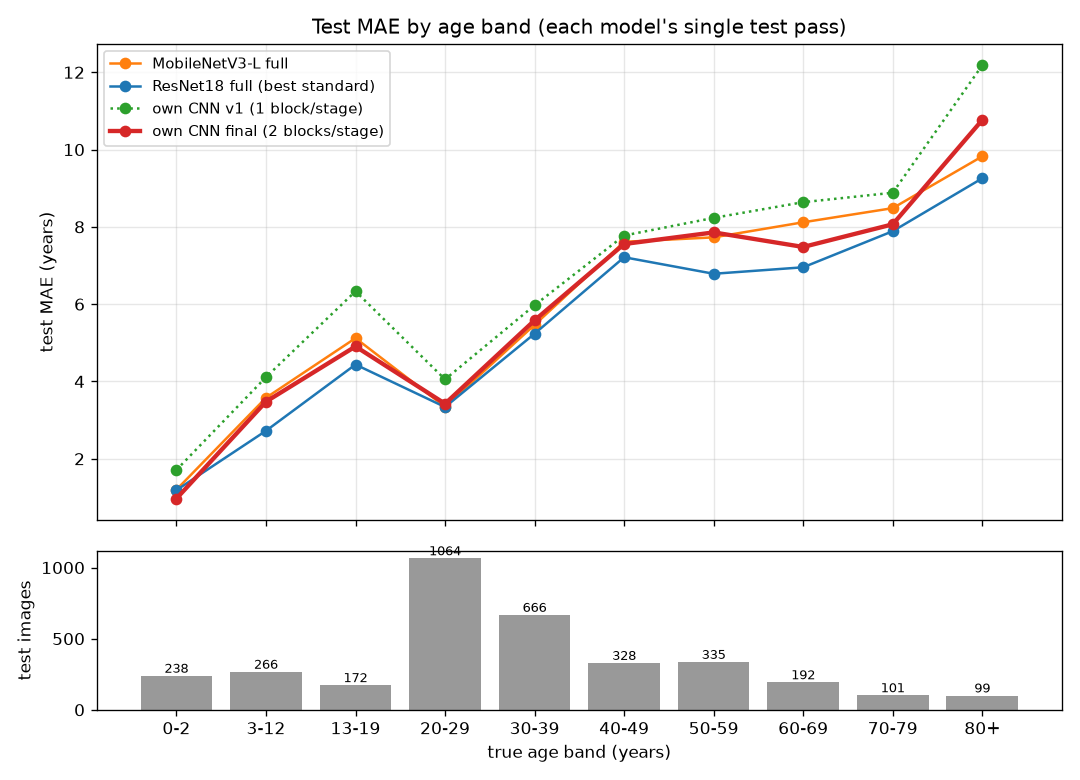
\includegraphics[width=\linewidth]{test_mae_by_age_own_vs_standard.png}
\caption{Test MAE per age band of the trained models (bottom: number of test images per band). Bands with few images (13--19, 70--79, 80+) have noisy MAEs.}
\label{fig:agemae}
\end{figure}

\begin{figure*}[t]
\centering
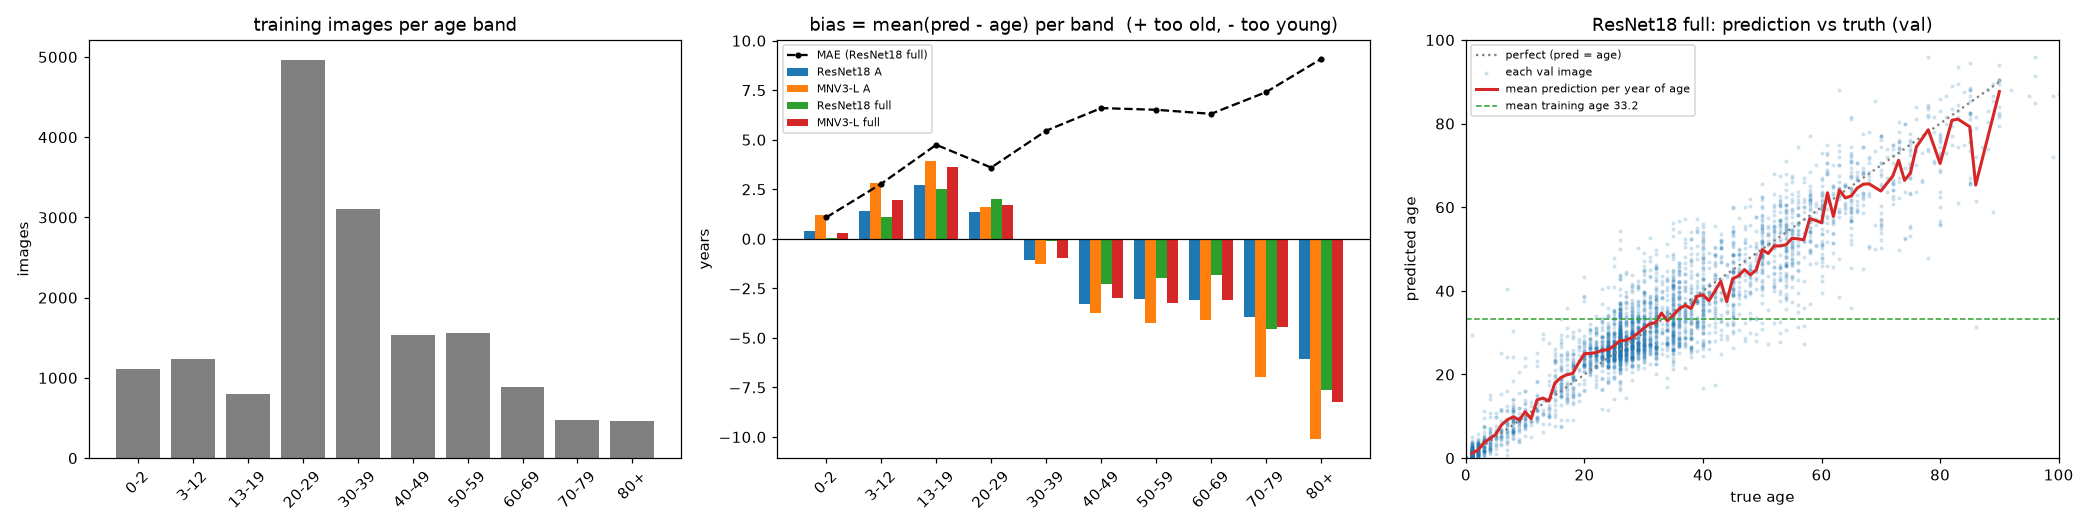
\includegraphics[width=0.95\textwidth]{error_by_age_val.png}
\caption{Age bias on the validation set. Left: training images per age band. Middle: signed bias $\mathrm{mean}(\hat{y}-y)$ per band for the four standard runs and the MAE of ResNet18 full (dashed). Right: ResNet18 predictions vs.\ true age; the red line (mean prediction per year of age) is pulled towards the training mean of 33.2 at both ends.}
\label{fig:valbias}
\end{figure*}

\textbf{Balancing does not help here.} We retrained ResNet18 (full) with each image's L1 loss weighted by $w_b = c/\sqrt{n_b}$, where $n_b$ is the number of training images in its age band and $c$ makes the mean weight 1 (weights from 0.61 for 20--29 to 2.01 for 80+). Validation MAE rose from 4.762 to 4.960, the mean of the 10 band MAEs rose from 5.357 to 5.409, and the bias at 80+ barely moved ($-7.61\to-7.19$). The weighted loss reduces the effective sample size by 13\,\% and the old-age error appears to be partly genuine ambiguity (and label heaping), not only a lack of examples. We kept the plain L1 loss. This run cost 2.62\,g and used validation data only.

\textbf{By gender and race.} Table~\ref{tab:groups} gives the test MAE per group. The differences between races are large even for the constant baseline (Black 10.6 vs.\ White 17.9 years) because age and race are confounded in UTKFace (e.g.\ 39\,\% of the 0--2 band is Asian, 72\,\% of the 80+ band is White). Groups with many children or young adults (Asian, Others) therefore have lower MAEs for every model. All three models rank the groups similarly (White and Black highest, Asian and Others lowest); our CNN's errors are 5--9\,\% higher than ResNet18's in every group, i.e.\ we see no group-specific disadvantage beyond its overall gap. Women have lower MAEs than men for all models, also partly because women dominate the younger bands.

\begin{table}[t]
\caption{Test MAE (years) per gender and race.}
\label{tab:groups}
\centering\footnotesize
\setlength{\tabcolsep}{3.5pt}
\begin{tabular}{@{}lrrrrr@{}}
\toprule
Group & $n$ & Mean & ResNet18 & MNV3-L & Own \\
 & & baseline & full & full & final \\
\midrule
Male & 1{,}802 & 15.82 & 4.97 & 5.28 & 5.39 \\
Female & 1{,}659 & 14.95 & 4.55 & 4.99 & 4.87 \\
\midrule
White & 1{,}474 & 17.89 & 5.26 & 5.55 & 5.73 \\
Black & 662 & 10.60 & 5.22 & 5.71 & 5.50 \\
Asian & 505 & 16.97 & 3.54 & 4.01 & 3.78 \\
Indian & 578 & 13.60 & 4.67 & 5.06 & 5.10 \\
Others & 242 & 14.35 & 3.35 & 3.61 & 3.52 \\
\bottomrule
\end{tabular}
\end{table}

% =====================================================================
\section{Discussion}
\textbf{What reduced the footprint.} (i) The images were decoded once into a 2.77\,GB uint8 cache kept on the GPU (built in 6\,s, 0.15\,Wh), so no epoch decoded JPEGs. (ii) bf16 mixed precision for all training. (iii) The learning-rate search ran on 4{,}000 images (2.2\,Wh for six short runs) instead of the full set. (iv) Every new piece of code was smoke-tested on 512 images (about 0.07\,Wh) before a full run. (v) Partial fine-tuning (A) halved the energy per epoch of the standard models, for 0.12--0.19 years of MAE. (vi) The test set was evaluated once per final model, and we stopped after the first acceptable model instead of tuning further. (vii) We did not train longer: the final model's validation curve was flat for its last 20 epochs.

\textbf{Trade-offs.} Our CNN reaches the target with 4$\times$ fewer parameters and FLOPs than ResNet18 and ties MobileNetV3 in MAE. For a one-off experiment, however, fine-tuning a pre-trained network was the cheaper way to an accurate model in this project, because the pre-training is already paid. Training from scratch pays off only if the model is used for many predictions, or if the pre-training cost is attributed to the user. On a GPU, low FLOPs do not guarantee low energy: dense $3\times3$ convolutions on few channels were cheaper than depthwise designs.

\textbf{Limitations.} (1) Every number comes from one seed; differences of about 0.2 years may partly be seed noise. (2) The improvement of our CNN changed depth and epochs together. (3) The final run's energies are upper bounds because another process shared the GPU. (4) The training faces all come from the same UTKFace alignment and the augmentation contains no zoom, so robustness to tighter or looser face crops was not measured; we expect the from-scratch model to be more sensitive to it than the ImageNet models, and random zoom augmentation (scale 0.8--1.2) would be the first fix. (5) Only byte-identical duplicates were detected; re-encoded near-duplicates may remain. (6) We planned to report the error on black-and-white vs.\ colour test images but did not save per-image test predictions, and re-running the test set only for this would break the one-test-pass rule. (7) The pre-training cost in Section~\ref{sec:results} is a rough estimate, not a measurement.

% =====================================================================
\section{Conclusion}
A small residual CNN trained from scratch (2.80\,M parameters, 374\,M MACs) reached a test MAE of 5.14 years on UTKFace and is acceptable under the assignment's definition, 8\,\% behind fully fine-tuned ResNet18 (4.77) and level with MobileNetV3-Large (5.14). The whole project used 72.0\,Wh and emitted 33.5\,g~\cotwoeq, every run measured. The cheapest acceptable result in \emph{training} \cotwo{} was not our model but a short fine-tuning of a pre-trained ResNet18; our model wins on size and inference energy and avoids the pre-training cost. On modern GPUs, measured energy, not MACs, should guide green model design.

\section*{Reproducibility}
Code, notebooks, the split file, all CodeCarbon logs and \texttt{results/results.csv} are in the project repository; the README lists the commands for every number. The final weights are \texttt{checkpoints/own\_cnn\_d2\_run02.pt} (11.2\,MB). Seed 655 everywhere.

\bibliographystyle{IEEEtran}
\bibliography{refs}

% =====================================================================
\appendices
\section{Additional Figures}

\begin{figure*}[t]
\centering
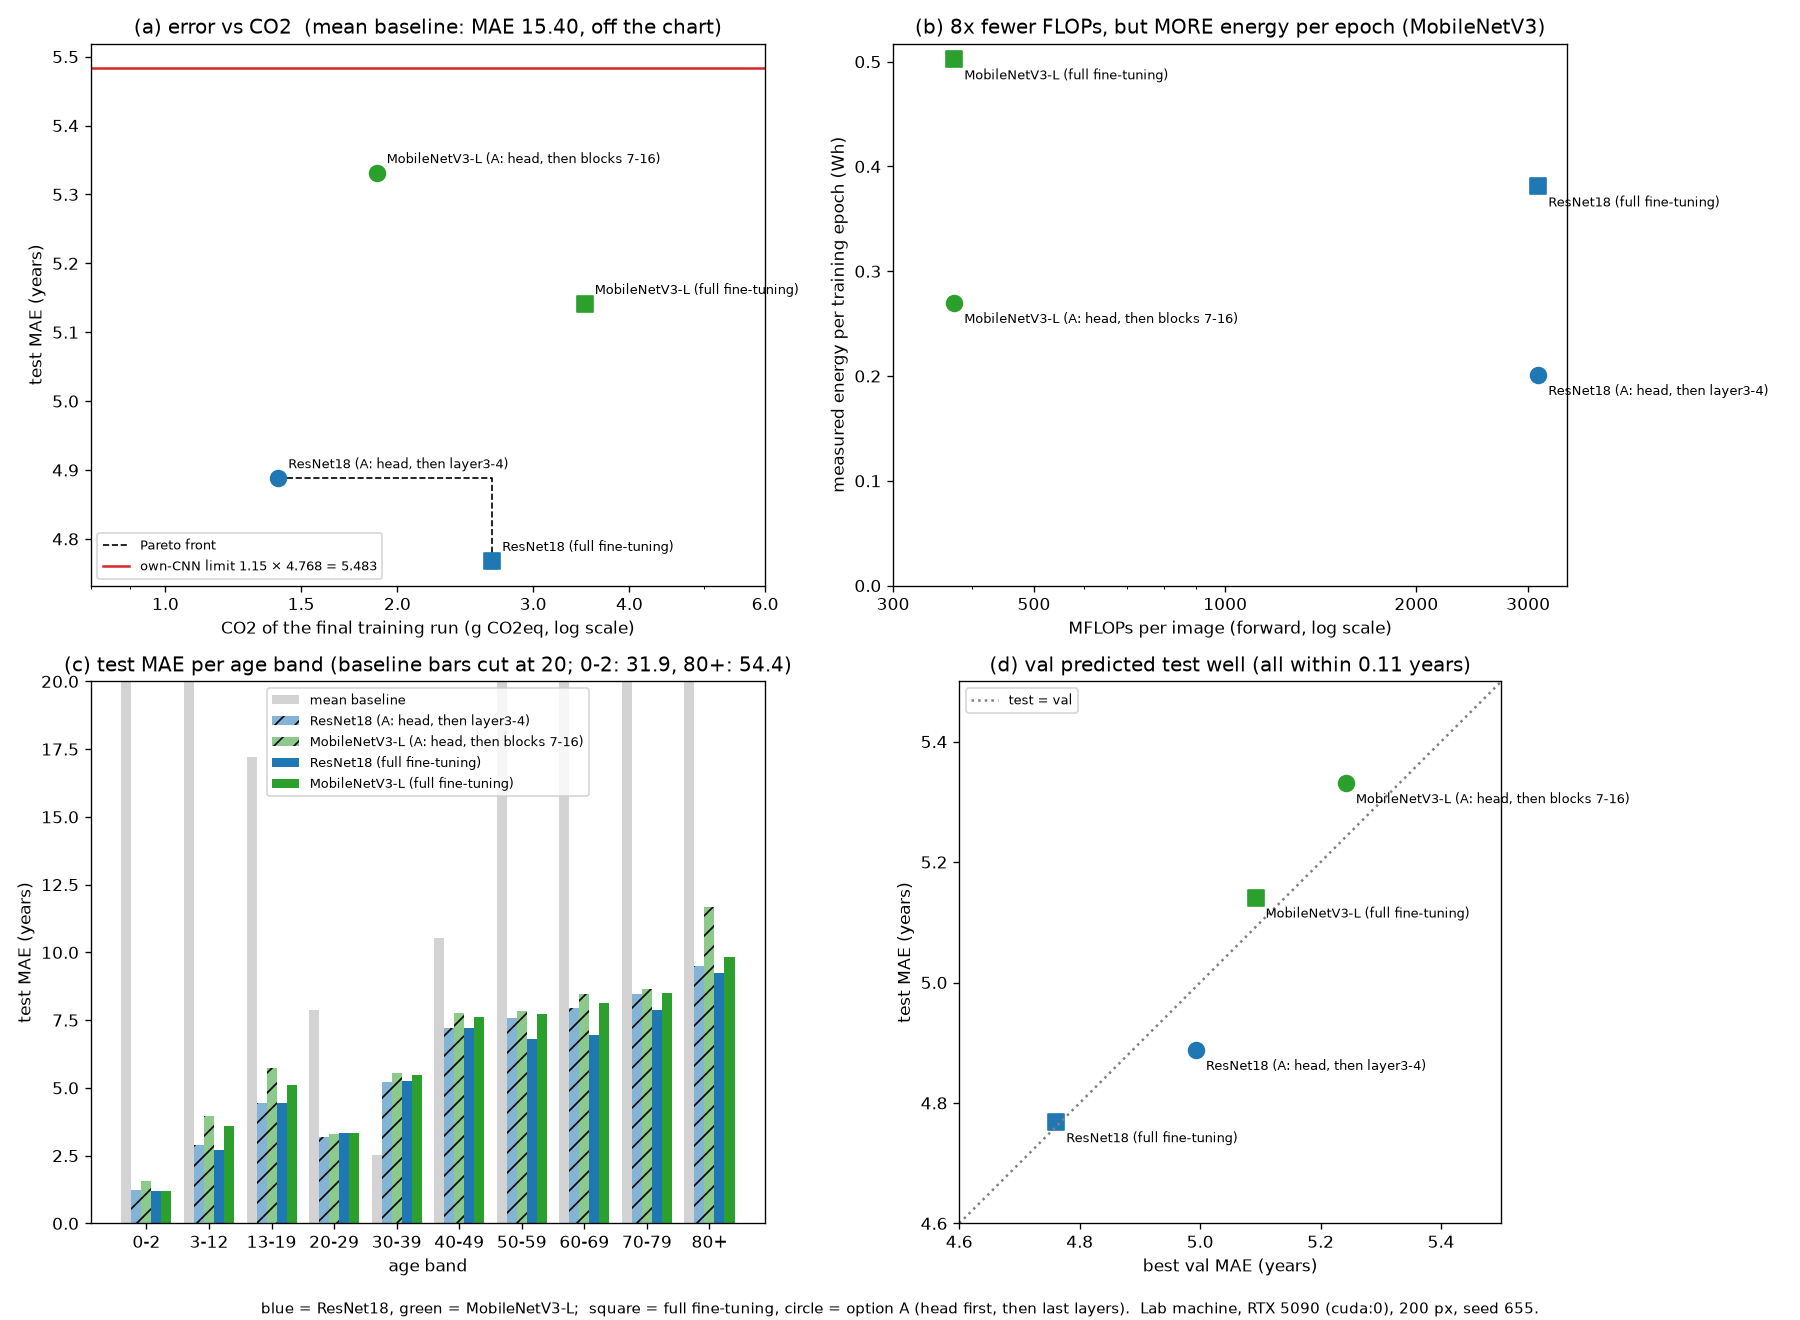
\includegraphics[width=0.85\textwidth]{findings_standard_models.png}
\caption{Standard models. (a) Test MAE vs.\ training \cotwo{} with the Pareto front; (b) MFLOPs per image vs.\ measured energy per training epoch: MobileNetV3-L has 8$\times$ fewer FLOPs but needs more energy; (c) test MAE per age band with the mean baseline (bars cut at 20); (d) validation vs.\ test MAE.}
\label{fig:findings}
\end{figure*}

\begin{figure*}[t]
\centering
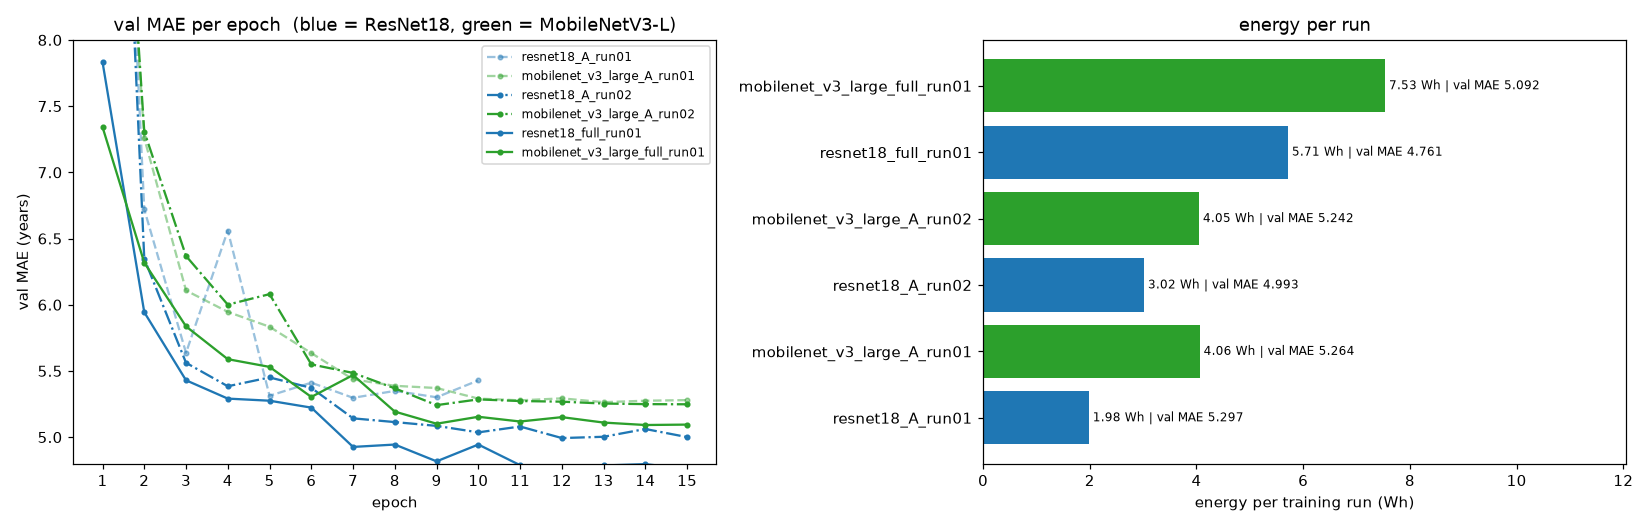
\includegraphics[width=0.85\textwidth]{compare_standard_runs.png}
\caption{Training curves of the four final standard-model runs (15 epochs, strategy A vs.\ full fine-tuning).}
\label{fig:stdcurves}
\end{figure*}

\begin{figure*}[t]
\centering
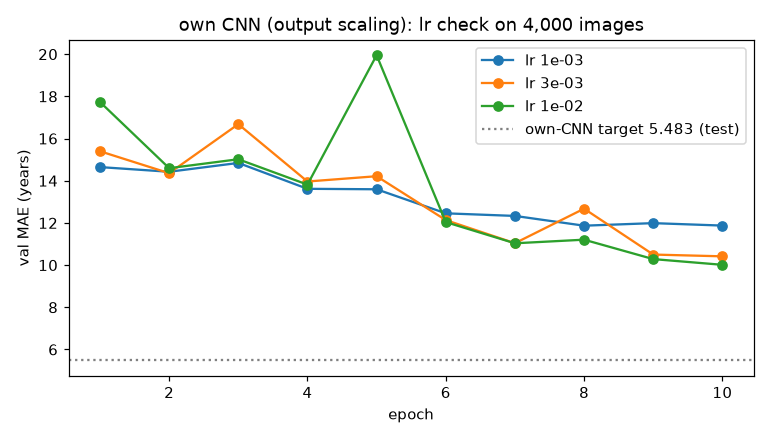
\includegraphics[width=0.6\textwidth]{own_cnn_lr_search2.png}
\caption{Learning-rate check of our CNN on 4{,}000 training images (10 epochs per rate, after the output-scaling fix).}
\label{fig:lrsearch}
\end{figure*}

\begin{figure*}[t]
\centering
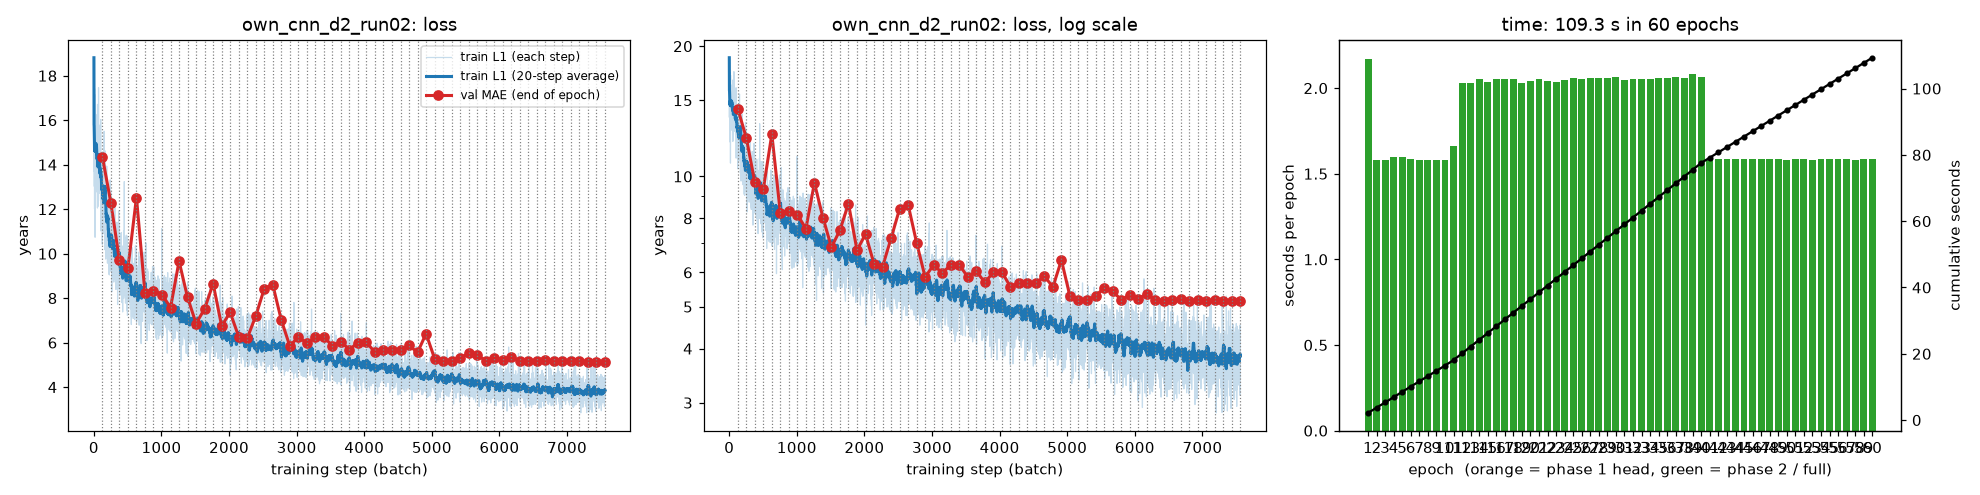
\includegraphics[width=\textwidth]{train_own_cnn_d2_run02.png}
\caption{Final CNN training run: loss per step (linear and log scale, red = validation MAE per epoch) and time per epoch. The slower epochs 12--40 coincide with another process on the GPU.}
\label{fig:d2train}
\end{figure*}

\begin{figure*}[t]
\centering
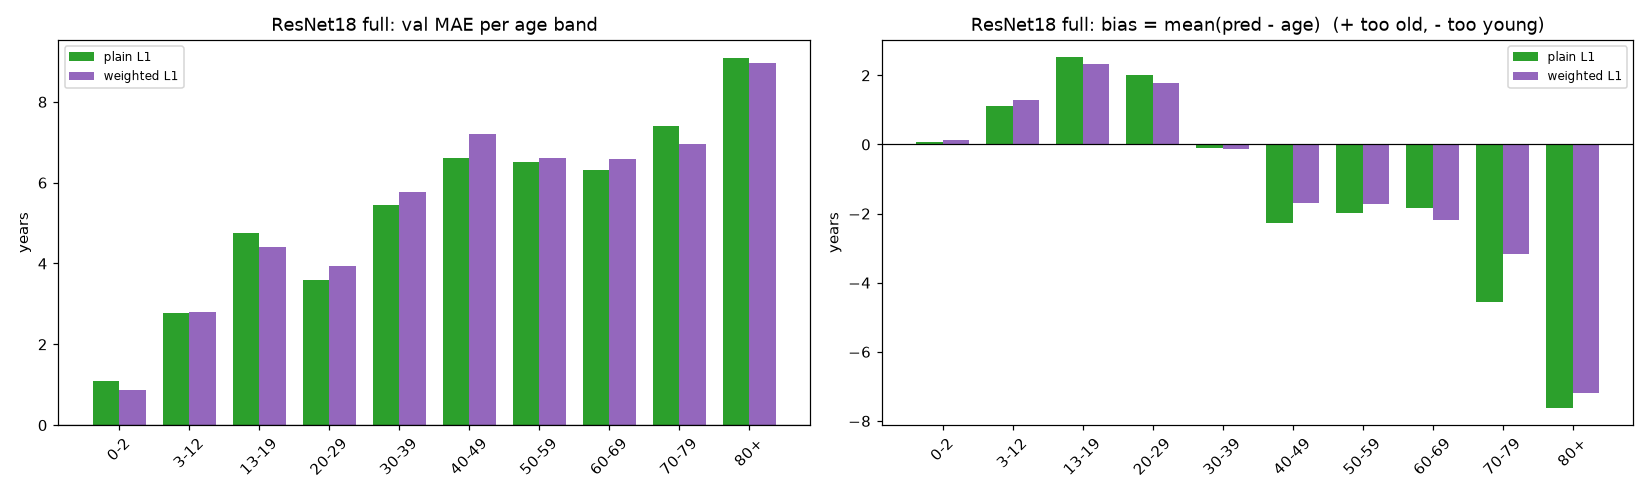
\includegraphics[width=\textwidth]{balanced_loss_vs_plain_val.png}
\caption{ResNet18 (full) with the plain L1 loss and with the $1/\sqrt{n_b}$-weighted L1 loss: validation MAE per age band (left) and signed bias per age band (right).}
\label{fig:balanced}
\end{figure*}

\end{document}
